% !TEX program = pdflatex
% !TEX root = manuscript.tex
% Statistics and Computing manuscript source.
% Springer Nature official template Version 3.1 (December 2024).
% Load before sn-jnl, which loads hyperref, to preserve external PDF links.
\RequirePackage{xr-hyper}
\documentclass[pdflatex,iicol,sn-mathphys-ay]{sn-jnl}
\usepackage[T1]{fontenc}
\usepackage[utf8]{inputenc}
\usepackage{amsmath,amssymb,amsfonts,amsthm,mathtools}
\usepackage{graphicx,booktabs,array,microtype}
\usepackage{placeins}
\usepackage{xurl}
\usepackage[nospread]{flushend}
% Compact spacing while retaining the journal's fonts and column geometry.
\makeatletter
\g@addto@macro\th@thmstyleone{\thm@preskip=8pt plus2pt minus1pt\relax\thm@postskip=8pt plus2pt minus1pt\relax}
\g@addto@macro\th@thmstyletwo{\thm@preskip=8pt plus2pt minus1pt\relax\thm@postskip=8pt plus2pt minus1pt\relax}
\g@addto@macro\th@thmstylethree{\thm@preskip=8pt plus2pt minus1pt\relax\thm@postskip=8pt plus2pt minus1pt\relax}
\setlength{\@fptop}{0pt}
\setlength{\@fpsep}{12pt}
\setlength{\@fpbot}{0pt plus1fil}
\setlength{\@dblfptop}{0pt}
\setlength{\@dblfpsep}{12pt}
\setlength{\@dblfpbot}{0pt plus1fil}
\makeatother
\setlength{\floatsep}{12pt plus2pt minus2pt}
\setlength{\textfloatsep}{10pt plus2pt minus2pt}
\setlength{\intextsep}{12pt plus2pt minus2pt}
\setlength{\dblfloatsep}{12pt plus2pt minus2pt}
\setlength{\dbltextfloatsep}{10pt plus2pt minus2pt}
% Moderate display spacing; keep the template's fonts and line spacing.
\AddToHook{cmd/normalsize/after}{%
  \setlength{\abovedisplayskip}{8pt plus2pt minus2pt}%
  \setlength{\belowdisplayskip}{8pt plus2pt minus2pt}%
}
\AtBeginDocument{\normalsize}
\providecommand{\burl}[1]{\url{#1}}
\hypersetup{colorlinks=true,linkcolor=blue,citecolor=blue,urlcolor=blue,filecolor=blue,bookmarksdepth=3,
  pdftitle={Optimal Subsampling for Regularized Linear Regression: A Generator-Function Framework},
  pdfauthor={Junchen Li, Ying-Ao Wang, Ye Zhang},
  pdfsubject={Data-conditional asymptotics and optimal row and column subsampling for spectral regression estimators}}
\theoremstyle{thmstyleone}
\newtheorem{theorem}{Theorem}
\newtheorem{lemma}{Lemma}
\newtheorem{proposition}{Proposition}
\newtheorem{corollary}{Corollary}
\theoremstyle{thmstylethree}
\newtheorem{definition}{Definition}
\newtheorem{assumption}{Assumption}
\theoremstyle{thmstyletwo}
\newtheorem{remark}{Remark}
\newtheorem{example}{Example}
\raggedbottom
\allowdisplaybreaks[2]
\newcommand{\bx}{\mathbf{x}}
\newcommand{\bX}{\mathbf{X}}
\newcommand{\bY}{\mathbf{Y}}
\newcommand{\bbeta}{\boldsymbol{\beta}}
\newcommand{\bSigma}{\boldsymbol{\Sigma}}
\newcommand{\cO}{\mathcal{O}}
\newcommand{\RR}{\mathbb{R}}
\newcommand{\EE}{\mathbb{E}}
\newcommand{\Var}{\mathrm{Var}}
\newcommand{\tr}{\mathrm{tr}}
\newcommand{\R}{\mathbb R}
\newcommand{\E}{\mathbb E}
\newcommand{\Prob}{\mathbb P}
\newcommand{\norm}[1]{\lVert#1\rVert}
\newcommand{\heading}[1]{\medskip\noindent\textbf{#1}\enspace}
\setlength{\emergencystretch}{2em}

% ORCID vector artwork adapted from the IMA class; no image file is required.
\usepackage{tikz}

\usetikzlibrary{svg.path}

\definecolor{orcidlogocol}{HTML}{A6CE39}
\tikzset{
  orcidlogo/.pic={
    \fill[orcidlogocol] svg{M256,128c0,70.7-57.3,128-128,128C57.3,256,0,198.7,0,128C0,57.3,57.3,0,128,0C198.7,0,256,57.3,256,128z};
    \fill[white] svg{M86.3,186.2H70.9V79.1h15.4v48.4V186.2z}
                 svg{M108.9,79.1h41.6c39.6,0,57,28.3,57,53.6c0,27.5-21.5,53.6-56.8,53.6h-41.8V79.1z M124.3,172.4h24.5c34.9,0,42.9-26.5,42.9-39.7c0-21.5-13.7-39.7-43.7-39.7h-23.7V172.4z}
                 svg{M88.7,56.8c0,5.5-4.5,10.1-10.1,10.1c-5.6,0-10.1-4.6-10.1-10.1c0-5.6,4.5-10.1,10.1-10.1C84.2,46.7,88.7,51.3,88.7,56.8z};
  }
}

%% Reciprocal of the height of the svg whose source is above.  The
%% original generates a 256pt high graphic; this macro holds 1/256.
\newcommand{\SCORCIDScale}{0.00390625}

%% We will compute the current X height to make the logo the right height
\newlength{\SCORCIDHeight}

\DeclareRobustCommand\ORCID[1]{%
\texorpdfstring{%
\setlength{\SCORCIDHeight}{\fontcharht\font`X}%
\href{https://orcid.org/#1}{\XeTeXLinkBox{\mbox{%
\begin{tikzpicture}[yscale=-\SCORCIDScale*\SCORCIDHeight,
xscale=\SCORCIDScale*\SCORCIDHeight,transform shape]
\pic{orcidlogo};
\end{tikzpicture}%
}}}}{}}

\graphicspath{{figure/}}
\setcitestyle{authoryear,round,aysep={},yysep={;}}
\externaldocument[supp-][nocite]{ESM_1}[ESM_1.pdf]


\begin{document}
\title[Optimal Subsampling for Regularized Linear Regression]{Optimal Subsampling for Regularized Linear Regression: A Generator-Function Framework}
% Corresponding-author identity has not yet been confirmed; no star is inferred.
\author[1]{\fnm{Junchen} \sur{Li}}\email{lijunchen@bit.edu.cn}
\author[1]{\fnm{Ying-Ao} \sur{Wang}\,\ORCID{0000-0001-8073-380X}}\email{wya@bit.edu.cn}
\author*[1,2]{\fnm{Ye} \sur{Zhang}\,\ORCID{0000-0003-4023-6352}}\email{ye.zhang@smbu.edu.cn}
\affil[1]{\orgdiv{School of Mathematics and Statistics}, \orgname{Beijing Institute of Technology}, \orgaddress{\city{Beijing}, \postcode{100081}, \country{China}}}
\affil[2]{\orgdiv{MSU-BIT-SMBU Joint Research Center for Applied Mathematics}, \orgname{Shenzhen MSU-BIT University}, \orgaddress{\city{Shenzhen}, \postcode{518172}, \country{China}}}
\abstract{We develop a data-conditional theory of row and column subsampling for
linear regression estimators defined by spectral generators. Effective-space
analysis permits rank-deficient designs, while local differentiability yields
complete influence functions and possibly degenerate central limit theorems.
Additional tail conditions give asymptotic expansions of the conditional mean,
covariance, and mean squared error. Comparing with sampled least squares
provides limits for changing regularization and same-sample tuning without
uniform derivative bounds. We also give verifiable conditions for
fixed-dimensional contrasts when the number of columns grows, derive optimal
importance probabilities with positive lower bounds, and verify the framework
for Nesterov acceleration, heavy ball with friction, and second-order
asymptotic regularization.
Numerical experiments compare row and column sampling probabilities, assess the first-order conditional MSE expansion, and examine approximation by least-squares comparison estimators constructed from the same sampling draws as regularization vanishes. Using actual recurrences and fixed-grid numerical flows with matching targets and influences, they show lower mean fixed-target approximation errors under influence sampling in the studied settings. Conditional Monte Carlo diagnostics quantify first-order MSE calibration and same-draw least-squares approximation across sampling budgets.}
\keywords{Subsampling, Ridge regression, Generator function, Optimal sampling, High-dimensional statistics}
\maketitle

% ============================================================
% SECTION 1: Introduction
% ============================================================
\section{Introduction}
\label{sec:introduction}

In a regression setting, observations $\{(X_{i1}, \ldots, X_{ip}, Y_i)\} \in \mathbb{R}^p \times \mathbb{R}$ for $i = 1, \ldots, n$ are used to fit a linear model
\begin{equation*}
    Y_i = \sum_{j=1}^{p} X_{ij}\beta_j + \varepsilon_i,
\end{equation*}
where $\varepsilon_i$ are i.i.d. random errors with
$\mathbb{E}[\varepsilon_i] = 0$ and $\mathbb{E}[\varepsilon_i^2] < \infty$.

Despite rapid advances in machine learning, the linear model continues to serve as a workhorse of statistical practice. Its popularity stems not only from interpretability and ease of implementation, but also from its role as a building block for more complex procedures. In large-scale applications---genomics, recommendation systems, text analysis, among others---the sheer volume of data makes it expensive or even infeasible to compute standard estimators using the full dataset. One natural remedy is \emph{subsampling}: rather than using all $n$ observations or all $p$ features, one makes $N$ draws with replacement and performs estimation using the resulting weighted sample. Here $N$ counts draws, including repeated selections, and need not be smaller than the number of available rows or columns. When the sampling probabilities and the sampled estimator can be computed efficiently, subsampling can reduce the cost of approximating the full-data estimator.

Uniform subsampling treats all data points equally, but can be inefficient when the design is heterogeneous. Data-dependent methods instead use quantities such as leverage scores to guide sampling; their approximation guarantees and statistical properties have been studied extensively~\citep{drineas2006sampling,ma2015statistical}. Optimal subsampling further selects probabilities for a specified estimation or prediction criterion. Influence-function methods provide a general route to asymptotically optimal probabilities~\citep{ting2018optimal}, while asymptotic analysis of least-squares sampling estimators yields probabilities that minimize suitable mean squared error criteria~\citep{ma2022asymptotic}. These results motivate studying how the appropriate influences and sampling criteria change with the regularization method.

A separate but equally important challenge arises when the dimensionality $p$ is comparable to or larger than $n$. If $X_n$ is rank deficient, the least-squares coefficient vector is not unique, although its minimum-norm representative $X_n^\dagger Y_n$ is always defined. Small positive singular values can also make this representative unstable. Regularization controls this sensitivity by modifying the inverse on the positive spectrum. Ridge regression adds an $\ell_2$ penalty to the least squares objective~\citep{hoerl1970ridge}; other approaches, such as the Lasso, impose sparsity-promoting penalties~\citep{tibshirani1996lasso}. The generator framework developed here concerns estimators that are linear in the responses for fixed tuning parameters.

The interaction between subsampling and regularization has already been studied for ridge regression. Existing work analyzes optimization error and statistical risk under classical and Hessian sketches~\citep{wang2018sketched}, high-dimensional risks under primal and dual sketching~\citep{liu2020ridge}, and optimal subsampling for high-dimensional ridge regression~\citep{li2024optimal}. Projected spectral regularization also has learning-rate guarantees for general filters under randomized sketches and Nystr\"om sampling~\citep{lin2020convergences}. Our objective is to develop a common data-conditional analysis for a broader class of spectral estimators under row and column importance sampling. We focus on complete influence expansions on the effective space of a possibly rank-deficient design, distinguish distributional limits from expansions of actual conditional moments, and state conditions for changing regularization and same-sample retuning.

Spectral regularization theory~\citep{engl1996regularization} and generator-based
formulations of linear regression~\citep{wang2024linear} provide the starting
point. OLS, ridge regression, Landweber iteration~\citep{landweber1951iteration},
and Showalter's method~\citep{showalter1967representation} share a generator
representation in which a scalar function acts on the Gram matrix. This
representation supports a common analysis while retaining the two sampling
mechanisms: column sampling perturbs the dual Gram matrix and uses the full
$X_n^\top$ to recover coefficients, whereas row sampling jointly perturbs the
Gram matrix and the response cross-product. Their different influence
functions are derived from the formal constructions in
Section~\ref{sec:formulation}.

\medskip
\noindent\textbf{Contributions.}
The main contributions of this paper are summarized as follows.
\begin{itemize}
    \item \textbf{A common statistical framework for two sampling mechanisms.}
    Complete influence functions account for dual-Gram sampling in the column
    scheme and for both Gram and cross-moment sampling in the row scheme.
    Local spectral assumptions are separated from the definition of a
    regularizing family, and all derivatives act on the effective space.
    \item \textbf{Distributional limits and conditional moment expansions.}
    Fixed-data central limit theorems allow degenerate covariance.
    Under explicit tail conditions, $L^2$ remainder bounds give asymptotic
    expansions of the conditional mean, covariance, and MSE.
    \item \textbf{Changing regularization and growing-column arrays.}
    Comparison with sampled least squares gives residual-based conditions for
    consistency and LS-centered limits. Separate results handle random tuning
    and fixed-dimensional contrasts when the number of columns grows.
    The parameter and zero-spectrum conditions are verified for accelerated
    and inertial generators.
    \item \textbf{Optimal importance probabilities with admissibility constraints.}
    We specialize the influence-function sampling principle~\citep{ting2018optimal}
    to the row and column spectral influences and fixed contrasts.
    The resulting oracle probabilities, their lower-bound-constrained solution,
    zero scores, and nonattainment are characterized, together with conditions
    under which the covariance criterion determines the leading conditional MSE.
\end{itemize}

\medskip
\noindent\textbf{Organization.}
The remainder of the paper is organized as follows. The next section reviews the related literature on subsampling, high-dimensional regression, sketching methods, and regularization theory. Section~\ref{sec:formulation} develops the generator-function framework and formulates row and column subsampling separately. Section~\ref{sec:theory} contains the main theoretical results for the two subsampling regimes, including asymptotic normality, asymptotic expansion, conditional mean and variance, and optimal subsampling probabilities. The final sections present numerical experiments and summarize the results and their scope. Appendix~\ref{app:core-proofs} contains the full proofs of the core results. Auxiliary lemmas, remaining proofs, and method-specific derivations are collected in the supplementary material.

% ============================================================
% SECTION 2: Related Work
% ============================================================
\section{Related Work}
\label{sec:literature}

Randomized numerical linear algebra provides sampling and sketching methods
for approximating regression problems~\citep{drineas2006sampling,woodruff2014sketching}.
\citet{ma2015statistical} study the statistical properties of
algorithmic leveraging. \citet{ma2022asymptotic} derive asymptotic
distributions for least-squares sampling estimators with arbitrary positive
probabilities, distinguishing approximation of the full-data estimator from
inference for the underlying model parameter. Their AMSE and EAMSE criteria
also yield optimal sampling rules. \citet{ahfock2021statistical}
analyze data-oblivious random projections, including finite-sample Gaussian
sketch results and a conditional central limit theorem. Our conditional
perspective is shared with this literature; here the objects are row and
column importance-sampled spectral estimators, and the assumptions for
distributional convergence are separated from those for actual conditional
moment expansions.

Optimal subsampling depends on the target and the admissible sampling class.
\citet{wang2019information} develop optimal subsampling for
large-sample logistic regression. \citet{ting2018optimal}
give a general influence-function approach for asymptotically linear
estimators, including lower bounds on inclusion probabilities and distinctions
between estimation and prediction objectives. For general smooth
M-estimation, \citet{wang2022replacement} derive conditional and unconditional
asymptotic distributions and compare optimal probabilities for sampling with
replacement and Poisson sampling, including variance criteria for fixed
linear transformations. Their framework uses a nonsingular population Hessian
and jointly growing data and subsample sizes. We apply the influence-function
principle to the complete spectral influences of both sampling schemes.
Proposition~\ref{prop:optimal_probabilities} optimizes the limiting contrast
covariance over independent sampling with replacement, with the generator
and contrast held fixed. It also covers zero scores and states conditions
under which this covariance determines the leading conditional MSE.

Regularized sketching already has substantial theory. \citet{wang2018sketched} analyze classical and Hessian sketches for ridge
regression, including their different bias--variance behavior. Hessian
sketches also underpin iterative approximation methods for constrained least
squares~\citep{pilanci2016iterative}. \citet{liu2020ridge}
study primal and dual ridge sketching in a proportional high-dimensional
regime. Their dual estimator has the same algebraic form as our ridge column
estimator after normalization, although the sketch distributions and
asymptotic regimes differ. \citet{lejeune2024asymptotics} characterize
first- and second-order asymptotic equivalences of regularized sketched
pseudoinverses in proportional-growth regimes, with applications to ridge
sketching. These random-matrix equivalents concern a different limit from
the conditional fluctuation and moment expansions studied here.

Beyond ridge, \citet{lin2020convergences} establish learning rates for
projected spectral regularization in Hilbert-space regression, including
randomized sketches and Nystr\"om sampling. Their results use source and
capacity conditions to control population learning error. Here we study
data-conditional fluctuations and complete influence-based sampling criteria
for row and column importance sampling.

For row subsampling, \citet{chen2022optimal} derive a ridge-specific
first-order expansion that includes a penalty-perturbation term, together
with a centered covariance formula. For column subsampling, \citet{li2024optimal} derive a
ridge-specific probability score by minimizing the trace of the inner
covariance matrix $V_c$ in their dual analysis. Remark~\ref{rem:ridge_specialization}
recovers the row ridge identities and distinguishes the column criterion
from the trace of the complete coefficient covariance used here.
The present framework extends the analysis to general spectral generators
on the effective space of a possibly rank-deficient design. It separates
distributional limits from expansions of actual conditional moments through
explicit tail conditions, and treats changing generators, dependent
same-sample retuning, and growing-column contrasts under their respective
assumptions. These extensions use the established influence-function
sampling principle and recover the row-ridge identities above as special cases.

The spectral representation itself is classical in inverse-problem
regularization~\citep{engl1996regularization} and has been developed for linear
regression by \citet{wang2024linear}. For accelerated methods,
\citet{kindermann2021optimal} relates Nesterov residuals to
Gegenbauer polynomials and analyzes regularization convergence. \citet{bot2022convergence} study spectral regularization and convergence
rates for heavy-ball and vanishing-damping flows. These works supply the
method-specific background for Section~\ref{subsec:accelerated_generator_verification}
and the supplement. Our verification there checks the additional conditions
needed to use those generators in the present subsampling theory.

% ============================================================
% SECTION 3: Problem Formulation
% ============================================================
\section{Problem Formulation}
\label{sec:formulation}

The linear model motivates the regression setting. The theory below conditions on the observed design and responses, so its sampling conclusions require no distributional assumptions on the regression errors. We first present the generator estimators and then analyze their approximation to full-data targets and the associated optimal sampling probabilities.

Throughout Sections~\ref{sec:formulation} and~\ref{sec:theory}, let $F_n$ be the sigma-field generated by the full data $(X_n,Y_n)$, the sampling probabilities for the scheme under consideration, and any tuning parameters fixed before its subsampling draws. Conditional on $F_n$, the draw indices are independent and have the stated sampling probabilities. A parameter retuned using those draws is not part of $F_n$. We use $Z_N=o_{p\mid F_n}(a_N)$ to mean that $\Prob(\|Z_N\|>\varepsilon a_N\mid F_n)\to_p0$ for every $\varepsilon>0$; $O_{p\mid F_n}(a_N)$ denotes conditional tightness in probability at scale $a_N$. Conditional convergence in distribution to a fixed law means that the conditional expectations of every bounded Lipschitz test function converge in probability to its expectation under that law.

\subsection{Spectral Generator Estimators}
\label{subsec:theoretical_framework}

Building on spectral formulations in inverse problems and linear regression~\citep{engl1996regularization,wang2024linear}, we formulate row and column subsampling for a common class of generator estimators.

\subsubsection{Definition of the Generator Function}
\label{subsubsec:generator_def}

We begin with the definition of a \emph{generator function}, which characterizes a broad family of linear regression estimators through spectral transformations.

\begin{definition}[Regularizing generator family]
\label{def:generator}
For the sampling scheme under consideration, fix an $F_n$-measurable
spectral bound $\Lambda_\star>0$, before the draws and independently of $\alpha$, such
that every full and sampled Gram spectrum lies in $[0,\Lambda_\star]$.
A family $g_\alpha$, indexed by admissible values in $(0,\bar\alpha]$
with zero as an accumulation point, with residual
$r_\alpha(\lambda)=1-\lambda g_\alpha(\lambda)$ is regularizing on this
window if
\begin{itemize}
\item[\textbf{(D1)}] $r_\alpha(\lambda)\to0$ as $\alpha\to0$ for every
fixed $\lambda\in(0,\Lambda_\star]$, along the admissible parameter values;
\item[\textbf{(D2)}] there is a constant $\gamma_1<\infty$ such that
$|r_\alpha(\lambda)|\le\gamma_1$ for all
$\lambda\in(0,\Lambda_\star]$ and all admissible $\alpha$.
\end{itemize}
Each method also specifies a finite value $g_\alpha(0)$.
\end{definition}

The notation $g_\alpha$ is used for each method, with the method identified by the surrounding text. We retain the cited literature's parameter conventions: the admissible values can form an interval or a specified grid, and the iteration count or stopping time is specified as a function of $\alpha$. Auxiliary parameters such as step size or damping are suppressed in the notation and are held fixed unless stated otherwise. The experimental calibration scale $\alpha_{\mathrm{exp}}$, introduced in Section~\ref{sec:experiments}, is distinct from this method-specific parameter. Once all parameters are fixed, we also write $g=g_\alpha$ in the fixed-generator theory.

\noindent Conditions \textbf{(D1)}--\textbf{(D2)} describe regularization
of the positive spectrum. They impose neither full rank nor a global
$C^2$ requirement. The statistical results below state their own local
smoothness and moment assumptions. In particular, the fixed-generator
results also apply to individual spectral functions that need not form
a family satisfying (D1)--(D2). Even when every generator is smooth,
(D1)--(D2) alone need not ensure consistency for a changing sequence of
generators; Assumption~\ref{ass:residual_window} supplies sufficient local
uniform residual control for consistency and an LS-centered central limit theorem.

\subsubsection{Spectral Representation}
\label{subsubsec:spectral_representation}
For a symmetric positive semidefinite Gram matrix $B=Q\Lambda Q^\top$, define
\[
 g_\alpha(B)=Q g_\alpha(\Lambda)Q^\top,
\]
where $Q$ is orthogonal and $g_\alpha$ acts on each diagonal entry of
$\Lambda$. The positive eigenvalues of $X_n^\top X_n$ and $X_nX_n^\top$
are $\lambda_1\ge\cdots\ge\lambda_\rho>0$, where
$\rho=\operatorname{rank}(X_n)$; their square roots are the nonzero singular
values of $X_n$.
At zero, use the method's prescribed finite value on every realization,
including rank-deficient sketches. OLS uses the Moore--Penrose convention
$g_\alpha(0)=0$; the other methods use their stated natural extensions.
The corresponding SVD formulas and full-rank special cases are given in
Supplementary Section~\ref{supp-supp:sec:classical_generators}.

\subsubsection{General Form of the Estimator}
\label{subsubsec:estimator_form}

Given a generator function $g_\alpha$, the corresponding class of linear regression estimators is defined as:
\begin{equation*}
    \widehat{\beta}_{\alpha}(n)
    = g_{\alpha}\!\left(X_n^{\top} X_n\right) X_n^{\top} Y_n,
\end{equation*}
where $X_n\in\RR^{n\times p}$ and $Y_n\in\RR^n$. We use the
unnormalized Gram matrix. The normalized form
$g_\alpha(X_n^\top X_n/n)X_n^\top Y_n/n$ is recovered by replacing the
generator with $\bar g_\alpha(\lambda)=n^{-1}g_\alpha(\lambda/n)$.
Method-specific parameter rescalings are recorded in Supplementary
Section~\ref{supp-supp:sec:classical_generators}.

\subsection{Column Subsampling via the Dual Generator Form}
\label{subsec:column_subsampling_framework}

Column sampling acts on the feature index through the dual Gram matrix.

\subsubsection{Column Sketching Matrix and Compressed Dual Gram Operator}
\label{subsubsec:column_sketching_matrix}
Let $i_1,\ldots,i_N$ be conditionally independent draws with fixed
$F_n$-measurable probabilities $\pi_j>0$, $\sum_{j=1}^p\pi_j=1$.
The sampling matrix $S\in\RR^{p\times N}$ has columns
$s_t=e_{i_t}/\sqrt{N\pi_{i_t}}$. The compressed design $\widehat X_N=X_nS$
has Gram matrix
\begin{equation}
 \widehat X_N\widehat X_N^\top=X_nSS^\top X_n^\top.
 \label{eq:compressed_dual_gram}
\end{equation}
Both this matrix and $X_nX_n^\top$ are convex combinations of
$\pi_j^{-1}(X_ne_j)(X_ne_j)^\top$, so one may take
\[
 \Lambda_\star=\max_{1\le j\le p}\frac{\|X_ne_j\|_2^2}{\pi_j}.
\]
The bound holds for every sketch, and the response vector $Y_n$ is unchanged.

\subsubsection{Primal--Dual Equivalence for Generator Estimators}
\label{subsubsec:dual_generator_representation}

The SVD gives the primal--dual identity
\begin{equation}
 g_\alpha(X_n^\top X_n)X_n^\top Y_n
 =X_n^\top g_\alpha(X_nX_n^\top)Y_n.
 \label{eq:intro_primal_dual_identity}
\end{equation}
Replacing its dual Gram matrix by \eqref{eq:compressed_dual_gram} defines
\begin{equation}
 \widetilde\beta_{\mathrm{col},\alpha}
 =X_n^\top g_\alpha(X_nSS^\top X_n^\top)Y_n.
 \label{eq:col_subsampled_generator}
\end{equation}
The full $X_n^\top$ recovers a coefficient vector in $\RR^p$;
setting $S=I_p$ recovers the full-data target.

\subsubsection{Column-Subsampled Estimators in the Generator Framework}
\label{subsubsec:column_subsampled_estimators}

Four classical choices illustrate \eqref{eq:col_subsampled_generator}; see
\citet[Section~3.2 and Table~1]{wang2025debiasing} for their spectral
representations. Accelerated and inertial methods are summarized in
Section~\ref{subsec:accelerated_generator_verification}.

\begin{example}[Ordinary least squares]\label{ex:subsampled_ols}
With $g_\alpha(\lambda)=\lambda^{-1}$ for $\lambda>0$ and $g_\alpha(0)=0$,
independently of $\alpha$, the estimator is
\begin{equation}
 \widetilde\beta_{\mathrm{OLS}}
 =X_n^\top(X_nSS^\top X_n^\top)^\dagger Y_n.
 \label{eq:subsampled_ols}
\end{equation}
It is defined for rank-deficient sketches and generally differs from
restricted-feature least squares $S(X_nS)^\dagger Y_n$.
\end{example}

\begin{example}[Ridge regression]\label{ex:subsampled_ridge}
For $\alpha>0$, $g_\alpha(\lambda)=(\lambda+\alpha)^{-1}$ and
$r_\alpha(\lambda)=\alpha/(\lambda+\alpha)$, including the natural value
$g_\alpha(0)=1/\alpha$. This yields the dual ridge sketching form
of \citet{liu2020ridge}, after accounting for Gram normalization;
see also \citet{li2024optimal} for optimal ridge subsampling.
\end{example}

\begin{example}[Landweber iteration]\label{ex:subsampled_landweber}
Fix $h>0$ before sampling, independently of $\alpha$, with
$0<h\Lambda_\star<2$. For $0<\alpha\le1$, set
$k=\lfloor1/\alpha\rfloor$ and
\[
 g_\alpha(\lambda)=\frac{1-(1-h\lambda)^k}{\lambda}\quad(\lambda>0),
 \qquad g_\alpha(0)=kh.
\]
The canonical choice $\alpha=1/k$ represents the same iterate.
The residual $(1-h\lambda)^k$ verifies (D1)--(D2) on the stated window;
see Supplementary Section~\ref{supp-supp:sec:classical_generators}.
\end{example}

\begin{example}[Showalter's method]\label{ex:subsampled_showalter}
For the continuous-time analogue of Landweber iteration, set
$t=1/\alpha$ and
\[
 g_\alpha(\lambda)=\frac{1-e^{-\lambda t}}{\lambda}\quad(\lambda>0),
 \qquad g_\alpha(0)=t.
\]
\end{example}
All four methods use the common estimator \eqref{eq:col_subsampled_generator}
and the assumptions of the relevant statistical theorem.

\subsection{Row Subsampling: Observation-Space Reweighting}
\label{subsec:row_subsampling_framework}

Let $I_1,\ldots,I_N$ be conditionally independent observation indices with
fixed probabilities $\Prob(I_t=i\mid F_n)=\nu_i>0$ and $\sum_i\nu_i=1$.
Define $S_{\mathrm{row}}\in\RR^{N\times n}$ to have $t$-th row
$e_{I_t}^\top/\sqrt{N\nu_{I_t}}$, and put
$W_{\mathrm{row}}=S_{\mathrm{row}}^\top S_{\mathrm{row}}$.
Joint reweighting of the design and response gives
\[
 \widetilde\beta_{\mathrm{row},\alpha}
 =g_\alpha(X_n^\top W_{\mathrm{row}}X_n)
       X_n^\top W_{\mathrm{row}}Y_n.
\]
Thus both the Gram matrix and the response cross-product are random.
The ridge specialization and its complete influence are given in
Remark~\ref{rem:ridge_specialization}; Sections~\ref{subsec:fixed_generator_theory}
and~\ref{subsec:retuning_fixed_target} treat fixed and retuned generators.

\section{Theoretical Results}\label{sec:theory}
We first establish a fixed-data theory, then distinguish changing
regularization, non-negligible retuning around a fixed target, and growing
column arrays. Throughout this section we abbreviate $X_n,Y_n$ by $X,Y$.
All fixed-data probabilities and moments are conditional on the quantities
specified before sampling; no distributional model for the responses is
imposed. The symbols $a_j$ and $x_i$ denote a column and a transposed row,
respectively. Norms are Euclidean for vectors, spectral for matrices unless
the subscript $F$ indicates the Frobenius norm. Conclusions about a full-data
estimator are statements about algorithmic approximation, not automatically
about a data-generating regression parameter.
Proof sketches accompany the core results below; their complete proofs are in
Appendix~\ref{app:core-proofs}. Technical details and auxiliary results are
in the supplementary material.

\subsection{Fixed-data theory for general generators}
\label{subsec:fixed_generator_theory}

The full-data approximation viewpoint follows the conditional analyses of
sampling and sketching estimators~\citep{ma2022asymptotic,ahfock2021statistical}.
The formulation below treats general spectral generators and both sampling
mechanisms on the effective space, with separate assumptions for conditional
CLTs and actual moment expansions.

Throughout this subsection, both $n$ and $p$ are fixed and $N\to\infty$.
All probabilities and expectations concern only the subsampling draws,
conditional on the full data and the quantities fixed before those draws.
Write $Y=(y_1,\ldots,y_n)^\top$, $a_j=X_{\cdot j}\in\RR^n$, $x_i=X_{i\cdot}^{\top}\in\RR^p$, and
\[
 \begin{aligned}
 H&=XX^\top,\qquad A=X^\top X,\qquad c=X^\top Y,\\
 \beta_g&=g(A)c=X^\top g(H)Y.
 \end{aligned}
\]
The equality follows from a singular-value decomposition of $X$. For $g=g_\alpha$, $\beta_g$ is the full-data estimator $\widehat\beta_\alpha(n)$ defined earlier, viewed as a fixed target conditional on the data.
For $g(t)=t^{-1}$ on $t>0$ and $g(0)=0$, the target is
$\beta_{\mathrm{LS}}=X^\dagger Y$, where $X^\dagger$ is the Moore--Penrose inverse.
If $X=0$, both estimators below vanish, and their conclusions are immediate.
We henceforth assume $X\ne0$.

\begin{assumption}[Fixed sampling (A0)]\label{ass:fixed_sampling}
The matrices $X,Y$, the generator $g$ and all its tuning parameters are fixed.
Column indices $J_1,\ldots,J_N$ are i.i.d.\ with
$\Prob(J_t=j)=\pi_j>0$, $\sum_j\pi_j=1$; alternatively, row indices
$I_1,\ldots,I_N$ are i.i.d.\ with
$\Prob(I_t=i)=\nu_i>0$, $\sum_i\nu_i=1$.
These probabilities do not depend on $N$.
The function $g$ is real and finite on every attainable spectrum and is
defined on open neighborhoods of the positive eigenvalues of $A$.
Its value at zero is fixed and finite. We use the method's natural finite
continuous extension when available; otherwise an explicit finite convention
must be specified. Ordinary least squares uses $g(0)=0$. This value is part
of the estimator and is held fixed across all sampled realizations.
\end{assumption}

The two schemes need not be performed jointly. Their estimators are
\begin{align}
 \widehat H&=\frac1N\sum_{t=1}^N\frac{a_{J_t}a_{J_t}^\top}{\pi_{J_t}},
 &\widetilde\beta_{\mathrm{col}}&=X^\top g(\widehat H)Y,
 \label{eq:fixed_column_estimator}\\
 \widehat A&=\frac1N\sum_{t=1}^N\frac{x_{I_t}x_{I_t}^\top}{\nu_{I_t}},
 &\widehat c&=\frac1N\sum_{t=1}^N\frac{x_{I_t}y_{I_t}}{\nu_{I_t}},
 \notag\\
 \widetilde\beta_{\mathrm{row}}&=g(\widehat A)\widehat c.
 \label{eq:fixed_row_estimator}
\end{align}
Zero columns or zero rows may be removed before specifying the probabilities.
Every nonzero row or column remains in the sampling population, including
those whose first-order influence is zero.

\begin{assumption}[Local differentiability (A1)]\label{ass:local_first}
The scalar function $g$ is differentiable at each distinct positive
eigenvalue of $A$, equivalently at each distinct positive eigenvalue of $H$.
\end{assumption}

\begin{assumption}[Quadratic scalar remainder (A2)]\label{ass:local_second}
In addition to (A1), for each distinct positive eigenvalue $\mu$ there are
$\epsilon_\mu>0$ and $C_\mu<\infty$ such that, whenever
$|t-\mu|\le\epsilon_\mu$,
\[
 |g(t)-g(\mu)-g'(\mu)(t-\mu)|\le C_\mu|t-\mu|^2.
\]
\end{assumption}

\begin{remark}[Strength of the local smoothness conditions]
Assumption (A1) requires differentiability only at the finitely many distinct
positive full-data eigenvalues; being $C^1$ on their neighborhoods is a
sufficient, stronger condition. Assumption (A2) follows if $g'$ is locally
Lipschitz there, and in particular if $g$ is locally $C^2$.
These conditions impose neither smoothness at zero nor full rank, and their
constants need not be uniform over tuning parameters in the fixed-generator
theorem. Changing parameters and growing dimensions are treated separately
below. Smoothness alone does not control exact moments on rare samples;
that is the role of (A3).
\end{remark}

All matrix derivatives below are taken on the fixed effective space
$\mathcal R_M=\operatorname{range}(M)$, with $M=H$ or $A$, and are extended
by zero on its orthogonal complement. Both $M$ and its sampled counterpart
leave this space invariant. Let $m=\lambda_{\min}^+(M)$.
Choose a fixed $0<\delta<m/2$ so that every interval
$[\mu-\delta,\mu+\delta]$ lies in a neighborhood where the differentiability
remainder in (A1), divided by $|t-\mu|$, is bounded.
For conclusions using (A2), choose $\delta$ small enough that its quadratic
bound also holds on all these intervals.
Define $G_N=\{\|\widehat M-M\|_2\le\delta\}$ for the scheme in question.
On $G_N$, the sampled matrix is positive definite on $\mathcal R_M$.

\begin{assumption}[Localized tail control (A3)]\label{ass:fixed_tail}
For the scheme and the locally admissible radius $\delta$ just specified,
\[
 N\,\E\!\left[\|\widetilde\beta-\beta_g\|_2^2
                 \mathbf{1}_{G_N^c}\right]\longrightarrow0.
\]
\end{assumption}

Under (A0)--(A1), (A3) remains valid at every smaller fixed, locally
admissible radius; see Supplementary Remark~\ref{supp-rem:fixed_tail_radius}.

For an orthonormal eigenbasis $U$ of $\mathcal R_M$, with positive
eigenvalues $\lambda_1,\ldots,\lambda_\rho$, define the effective-space derivative by
\[
 \begin{aligned}
 Dg_M[E]&=U\{\mathcal L_g\circ(U^\top EU)\}U^\top,\\
 (\mathcal L_g)_{ab}&=
 \begin{cases}
 \dfrac{g(\lambda_a)-g(\lambda_b)}{\lambda_a-\lambda_b},&\lambda_a\ne\lambda_b,\\[3pt]
 g'(\lambda_a),&\lambda_a=\lambda_b.
 \end{cases}
 \end{aligned}
\]
This is the classical divided-difference form of the matrix-function
Fr\'echet derivative; see \citet[Chapter~3]{higham2008functions}.
Supplementary Lemma~\ref{supp-lem:local_matrix} gives a self-contained proof of its local expansion
under (A1) and the quadratic remainder under (A2), including repeated
eigenvalues. Supplementary Lemma~\ref{supp-lem:finite_atoms} supplies the
sampling moment, concentration, and positive-eigenvalue bounds.



Define the unweighted influence vectors by
\begin{align*}
 u_j&=X^\top Dg_H[a_ja_j^\top]Y,\\
 v_i&=Dg_A[x_ix_i^\top]c+g(A)x_iy_i.
\end{align*}
Write $\bar u=\sum_j u_j$ and $\bar v=\sum_i v_i$.
Their one-draw covariance matrices are
\begin{align*}
 \Omega_{\mathrm{col}}&=\sum_j\frac{u_ju_j^\top}{\pi_j}-\bar u\bar u^\top,
 \\
 \Omega_{\mathrm{row}}&=\sum_i\frac{v_iv_i^\top}{\nu_i}-\bar v\bar v^\top.
\end{align*}
For either scheme, write $s_i=u_i$ or $v_i$, and $\varpi_i=\pi_i$ or $\nu_i$.
With the corresponding draw indices $K_t$, put
\[
 Z_N=\frac1N\sum_{t=1}^N
       \left(\frac{s_{K_t}}{\varpi_{K_t}}-\sum_i s_i\right).
\]
Exactly, $\E Z_N=0$ and $\operatorname{Cov}(Z_N)=\Omega/N$.

\begin{theorem}[Fixed-data expansion and moments]\label{thm:fixed_generator}
Under (A0)--(A1), each scheme admits a remainder $R_N=o_p(N^{-1/2})$ such that
\[
 \begin{aligned}
 \widetilde\beta-\beta_g&=Z_N+R_N,\\
 \sqrt N(\widetilde\beta-\beta_g)&\Longrightarrow N_p(0,\Omega).
 \end{aligned}
\]
The covariance $\Omega$ may be singular or zero.
Under (A2), $R_N=O_p(N^{-1})$.
Under (A1) and (A3), the stronger moment statement
$\E\|R_N\|_2^2=o(N^{-1})$ holds, and hence
\begin{align*}
 \E\widetilde\beta&=\beta_g+o(N^{-1/2}),\\
 \operatorname{Cov}(\widetilde\beta)&=\Omega/N+o(N^{-1}),\\
 \E\|\widetilde\beta-\beta_g\|_2^2
     &=\tr(\Omega)/N+o(N^{-1}). 
\end{align*}
Under (A2) and (A3), the mean satisfies
$\E\widetilde\beta=\beta_g+O(N^{-1})$.
Vector and matrix remainders are understood in any fixed-dimensional norm.
\end{theorem}
\begin{proof}[Proof sketch]
Write $B_N=\widehat M-M$ and, for rows, $d_N=\widehat c-c$.
On $G_N$, expansion on the fixed effective space gives the linear term
$Z_N$; the row remainder also contains a term bounded by
$C\|B_N\|_2\|d_N\|_2$.
The finite-atom moment bounds give $R_N=o_p(N^{-1/2})$ under (A1)
and $R_N=O_p(N^{-1})$ under (A2).
The i.i.d.\ influence central limit theorem gives the possibly degenerate
Gaussian limit.
For the moment expansions, fourth-moment bounds control the remainder on $G_N$,
while (A3) and exponential concentration control its complement, yielding
$\E\|R_N\|_2^2=o(N^{-1})$.
Cauchy--Schwarz then gives the stated mean, covariance, and MSE expansions.
Under (A2), the good-event mean remainder is $O(N^{-1})$; (A3) and the
exponential probability bound make its bad-event contribution $o(N^{-1})$.
The complete proof is in Appendix~\ref{app:proof-fixed-generator}.
\end{proof}

\begin{remark}\label{rem:fixed_moment_scope}
A probability remainder alone does not justify taking expectations.
Moreover, (A2)--(A3) do not assert $\E\|R_N\|_2^2=O(N^{-2})$ globally:
(A3) controls the bad-event second moment only at order $o(N^{-1})$.
In particular, $\Omega=0$ yields MSE $o(N^{-1})$, not automatically
$O(N^{-2})$. Stronger tail control is needed for the latter rate.
Random retuning after subsampling, probabilities depending on $N$, and
growing $n$ or $p$ require additional analysis and are outside this theorem.
\end{remark}

\begin{proposition}[A checkable tail condition]\label{prop:fixed_tail_growth}
For the chosen fixed probabilities, let $[0,B]$ contain every attainable
Gram spectrum. If $g(0)$ is finite and
$|g(t)|\le C(1+t^{-q})$ for $0<t\le B$, with fixed $q\ge0$, then (A3)
holds for every fixed positive radius.
\end{proposition}
The proof is given in Supplementary Appendix~\ref{supp-supp:proof-fixed-tail}.

The following optimization specializes the influence-function principle of
\citet{ting2018optimal} to the influences above and a fixed
contrast. Related AMSE-based optimization for least-squares sampling appears
in \citet{ma2022asymptotic}. We characterize the minimizers on the relevant
probability domains, including cases with zero influence scores.

\begin{proposition}[Optimal probabilities for fixed contrasts]
\label{prop:optimal_probabilities}
Fix the generator, its parameters, and a contrast matrix $L\in\RR^{d\times p}$
while comparing probabilities. Let $s_i$ be the appropriate influences,
$w_i=\|Ls_i\|_2$, and let $\varpi$ denote the candidate probabilities.
The trace of the limiting contrast covariance is
\[
 \begin{aligned}
 Q_L(\varpi)&=\tr(L\Omega L^\top)\\
   &=\sum_i\frac{w_i^2}{\varpi_i}-\left\|\sum_i Ls_i\right\|_2^2.
 \end{aligned}
\]
If all $w_i>0$, its unique minimizer over strictly positive probabilities
is $\varpi_i^*=w_i/\sum_jw_j$.
If all $w_i=0$, every feasible probability vector is optimal.
If some but not all scores vanish, the positive-probability domain has
infimum $(\sum_iw_i)^2-\|\sum_iLs_i\|_2^2$, but no minimizer.

For fixed lower bounds $\ell_i>0$ with $\sum_i\ell_i\le1$,
the case $\sum_i\ell_i=1$ has the sole feasible vector $\varpi=\ell$.
If $\sum_i\ell_i<1$ and some $w_i>0$, the unique minimizer is
\[
 \varpi_i^*=\max\{\ell_i,\tau w_i\},
\]
where $\tau>0$ uniquely solves $\sum_i\max\{\ell_i,\tau w_i\}=1$.
If all scores vanish, every feasible vector is
optimal; the normalization equation then has no solution when
$\sum_i\ell_i<1$ and is not used.
\end{proposition}
Cauchy--Schwarz gives the unconstrained score rule, and the KKT conditions
give its lower-bound-constrained form. The complete proof is in
Appendix~\ref{app:proof-optimal-probabilities}.

Taking $L=I_p$ gives coefficient A-optimality.
Under (A0)--(A1) at the selected probabilities, the objective in the
proposition is the covariance trace of the Gaussian limit.
For this objective to determine the leading term of the conditional contrast
MSE, the following projected tail condition suffices at each fixed candidate
probability vector:
\begin{equation}\label{eq:fixed_contrast_tail}
 N\E\!\left[\|L(\widetilde\beta-\beta_g)\|_2^2
                    \mathbf{1}_{G_N^c}\right]\longrightarrow0.
\end{equation}
Under (A0)--(A1) and \eqref{eq:fixed_contrast_tail},
\[
 \E\|L(\widetilde\beta-\beta_g)\|_2^2
       =Q_L(\varpi)/N+o(N^{-1}).
\]
The proof is in Supplementary Appendix~\ref{supp-supp:proof-contrast-mse}.
The vector condition (A3) implies \eqref{eq:fixed_contrast_tail}, and
Proposition~\ref{prop:fixed_tail_growth} supplies a sufficient check for (A3).
These tail conditions are verified at each fixed candidate probability vector.
The lower bounds and the selected probabilities remain fixed as $N$ grows.
Nonzero atoms with zero score remain in the sampling population, preserving
$H$, $A$, and the target. The generator $g$ and its step size are held fixed
throughout this optimization.

\begin{remark}[Ridge specialization and related criteria]
\label{rem:ridge_specialization}
For fixed $\alpha>0$, put
\[
 \begin{aligned}
 G&=(A+\alpha I_p)^{-1},\qquad K=(H+\alpha I_n)^{-1},\\
 \beta_\alpha&=Gc=X^\top KY.
 \end{aligned}
\]
Both inverses exist even when $X$ is rank deficient. Writing
$e_\alpha=Y-X\beta_\alpha$, the inverse derivative
$Dg_M[E]=-(M+\alpha I)^{-1}E(M+\alpha I)^{-1}$ gives
\[
 v_i=Gx_i e_{\alpha i},\qquad
 \bar v=GX^\top e_\alpha=\alpha G\beta_\alpha.
\]
Consequently,
\begin{equation}\label{eq:ridge_row_covariance}
 \Omega_{\rm row}
 =G\left\{\sum_i\frac{e_{\alpha i}^2x_ix_i^\top}{\nu_i}
       -\alpha^2\beta_\alpha\beta_\alpha^\top\right\}G.
\end{equation}
This recovers the centered row-ridge covariance of
\citet{chen2022optimal}. The penalty-perturbation term in
Corollary~\ref{cor:row_ridge} also appears in their ridge expansion;
the joint-limit discussion below retains its dependence on the sampling
score when the penalty is selected from the same sketch.

For columns, the complete coefficient influence is
$u_j=-\beta_{\alpha j}X^\top Ka_j$. Thus, for $L=I_p$, the two scores in
Proposition~\ref{prop:optimal_probabilities} become
\begin{equation}\label{eq:ridge_complete_scores}
 \begin{aligned}
  w_i^{\rm row}&=|e_{\alpha i}|\,\|Gx_i\|_2,\\
  w_j^{\rm col}&=|\beta_{\alpha j}|\,\|X^\top Ka_j\|_2.
 \end{aligned}
\end{equation}
Equation (2.10) of \citet{li2024optimal} instead gives the score
$|\beta_{\alpha j}|\|a_j\|_2$: their $\tr(V_c)$ criterion is proportional,
by a factor independent of the probabilities, to
$\sum_j\beta_{\alpha j}^2\|a_j\|_2^2/\pi_j$.
The complete coefficient criterion uses $\|X^\top Ka_j\|_2^2$ in this sum,
with the probability-independent centering term subtracted.
The transformation $X^\top K$ cannot in general be omitted when minimizing
that trace. The zero-score and positive-lower-bound cases follow the conventions of Proposition~\ref{prop:optimal_probabilities}.
\end{remark}


\subsection{Least-squares limits and changing regularization}
\label{subsec:ls_limits}

Continue to condition on fixed finite data and fixed positive sampling probabilities.
We write $\widehat\beta_{g,C}=\widetilde\beta_{\rm col}$ and
$\widehat\beta_{g,R}=\widetilde\beta_{\rm row}$ for the estimators in
\eqref{eq:fixed_column_estimator}--\eqref{eq:fixed_row_estimator}, and make
the dependence on $N$ explicit in $\widehat H_N,\widehat A_N,\widehat c_N$.
The generators $g_N$ may now change with $N$; no uniform derivative bounds are imposed.
Write $\beta_{\rm LS}=X^\dagger Y$, $P=X^\dagger X$, and
$e=Y-X\beta_{\rm LS}$. The same-draw comparison estimators are
\begin{equation*}
 \begin{aligned}
 \widehat\beta_{{\rm LS},C}&=X^\top\widehat H_N^\dagger Y,\\
 \widehat\beta_{{\rm LS},R}&=\widehat A_N^\dagger\widehat c_N.
 \end{aligned}
\end{equation*}
In particular, the column comparison is the dual-generator estimator, not
$S(XS)^\dagger Y=SS^\top X^\top\widehat H_N^\dagger Y$.

\begin{assumption}[Residual approximation on a positive spectral window (A4)]
\label{ass:residual_window}
For $X\ne0$, let $m=\lambda_{\min}^+(XX^\top)$,
$M_{\max}=\norm{XX^\top}_2$, and $I=[m/2,M_{\max}+m/2]$.
Choose a fixed $0<\delta<m/2$, for example $\delta=m/4$, and define
\[
 I_\delta=\bigcup_{\mu\in\sigma_+(XX^\top)}[\mu-\delta,\mu+\delta],
\]
where $\sigma_+(XX^\top)$ is the set of distinct positive eigenvalues.
The residual window $\mathcal W$ may be either $I$ or $I_\delta$;
the default choice, including the method-specific verifications below,
is $\mathcal W=I$.
Each $g_N$ is fixed before the draws, is defined on $\mathcal W$, and has
finite values at all attainable sample eigenvalues, including its
prescribed value at zero. Define
\[
 \rho_N=\sup_{\lambda\in\mathcal W}|1-\lambda g_N(\lambda)|.
\]
For consistency assume $\rho_N\to0$; for the least-squares-centered central
limit theorem assume $\sqrt N\,\rho_N\to0$.
\end{assumption}

\begin{assumption}[Tail control for changing generators (A5)]
\label{ass:ls_tail}
Using the same $\delta$ as in Assumption~\ref{ass:residual_window}, set
$G_{C,N}=\{\norm{\widehat H_N-H}_2\le\delta\}$ and
$G_{R,N}=\{\norm{\widehat A_N-A}_2\le\delta\}$.
For the scheme $\mathsf{s}\in\{C,R\}$ under consideration, assume
\begin{equation}\label{eq:ls_tail}
 N\E\!\left[\norm{\widehat\beta_{g_N,\mathsf{s}}-\beta_{\rm LS}}^2
                  \mathbf{1}_{G_{\mathsf{s},N}^c}\right]\longrightarrow0.
\end{equation}
\end{assumption}

The radius transfer in Supplementary Remark~\ref{supp-rem:fixed_tail_radius} concerns fixed
generators; it is not assumed for changing or random generators.

\begin{theorem}[Asymptotic equivalence to sampled least squares]
\label{thm:ls_equivalence}
Under the data and sampling clauses of Assumption~\ref{ass:fixed_sampling},
the consistency part of
Assumption~\ref{ass:residual_window} implies
\[
 \widehat\beta_{g_N,\mathsf{s}}-\beta_{\rm LS}
       =O_p(N^{-1/2})+O_p(\rho_N)=o_p(1).
\]
Its stronger, root-$N$ part implies
\begin{equation}\label{eq:ls_clt}
 \sqrt N(\widehat\beta_{g_N,\mathsf{s}}-\beta_{\rm LS})
       \ \Longrightarrow\ N_p(0,\Omega_{{\rm LS},\mathsf{s}}),
\end{equation}
where degenerate covariance matrices are allowed and
\begin{align*}
 \Omega_{{\rm LS},C}
  &=\sum_j\frac{\beta_{{\rm LS},j}^2}{\pi_j}
       P_{\cdot j}P_{\cdot j}^\top-\beta_{\rm LS}\beta_{\rm LS}^\top,
       \\
 \Omega_{{\rm LS},R}
  &=A^\dagger\left(\sum_i\frac{e_i^2}{\nu_i}x_ix_i^\top\right)A^\dagger.
\end{align*}
The root-$N$ condition together with Assumption~\ref{ass:ls_tail} also gives
\begin{align}
 \E\widehat\beta_{g_N,\mathsf{s}}&=\beta_{\rm LS}+o(N^{-1/2}),\nonumber\\
 \operatorname{Cov}(\widehat\beta_{g_N,\mathsf{s}})
      &=\Omega_{{\rm LS},\mathsf{s}}/N+o(N^{-1}),\label{eq:ls_exact_moments}\\
 \E\norm{\widehat\beta_{g_N,\mathsf{s}}-\beta_{\rm LS}}^2
      &=\tr(\Omega_{{\rm LS},\mathsf{s}})/N+o(N^{-1}).\nonumber
\end{align}
If instead the stronger rate $\rho_N=O(N^{-1})$ holds together with
Assumption~\ref{ass:ls_tail}, the bias is $O(N^{-1})$.
\end{theorem}
\begin{proof}[Proof sketch]
On the good event, the full and sampled effective spaces agree, and the
residual bound compares the changing-generator estimator with sampled
least squares at order $\rho_N$, without derivative bounds on $g_N$.
An effective-space inverse expansion gives the sampled-LS influence sum;
the finite-support central limit theorem yields the displayed covariance
and distributional limit. Assumption~\ref{ass:ls_tail} additionally controls
the squared comparison error on rare samples, giving the exact moment
expansions. The stronger residual rate gives the stated bias order.
The complete proof is in Appendix~\ref{app:proof-ls-equivalence}.
\end{proof}

\begin{proposition}[A verifiable envelope for A5]\label{prop:tail_envelope}
In the fixed-data setting, suppose a deterministic $K_N\ge1$ bounds
$|g_N(\lambda)|$ at every attainable positive sample eigenvalue and
$\log K_N=o(N)$. For column sampling also require $|g_N(0)|\le K_N$.
Then Assumption~\ref{ass:ls_tail} holds. The same statement applies to random
generators if the deterministic envelope holds for every realization.
\end{proposition}
The proof is given in Supplementary Appendix~\ref{supp-supp:proof-tail-envelope}.

If $|1-\lambda g_N(\lambda)|\le C$ uniformly at all attainable positive
sample eigenvalues, Supplementary Lemma~\ref{supp-lem:finite_atoms} bounds the positive-spectrum
gain by $CN$. Only the column zero-spectrum gain then needs separate control.
This explains why small probabilities of rank loss cannot simply be ignored
when the regularization parameter tends to its unregularized limit.

\begin{corollary}[Random tuning toward the LS target]\label{cor:random_ls_tuning}
Let a measurable random generator, possibly chosen using the same draws,
be finite at every attainable sample eigenvalue, including its prescribed
value at zero, and have a measurable residual bound $\widehat\rho_N$ on
the same fixed window $\mathcal W$ as in
Assumption~\ref{ass:residual_window}. Use the corresponding good events
$G_{\mathsf{s},N}$ with that assumption's choice of $\delta$.
Then $\widehat\rho_N=o_p(1)$ gives consistency, and
$\sqrt N\,\widehat\rho_N=o_p(1)$ gives \eqref{eq:ls_clt}.
For the exact moments in \eqref{eq:ls_exact_moments}, sufficient conditions are
Assumption~\ref{ass:ls_tail} and
\begin{equation}\label{eq:random_tuning_l2}
 N\E[\widehat\rho_N^2\mathbf{1}_{G_{\mathsf{s},N}}]\longrightarrow0.
\end{equation}
For the bias alone, Assumption~\ref{ass:ls_tail} and
$\E[\widehat\rho_N\mathbf{1}_{G_{\mathsf{s},N}}]=O(N^{-1})$ suffice for an $O(N^{-1})$ bound.
The latter first-moment condition does not replace \eqref{eq:random_tuning_l2}
for covariance conclusions.
\end{corollary}
The proof is given in Supplementary Appendix~\ref{supp-supp:proof-random-tuning}.

\subsection{Non-negligible retuning around a fixed regularized target}
\label{subsec:retuning_fixed_target}
The following inverse-filter expansion retains the parameter perturbation
when it contributes at first order around a fixed target.

\begin{theorem}[Row expansion with a retuned parameter]\label{thm:row_expansion}
Let the data and sampling scheme satisfy Assumption~\ref{ass:fixed_sampling}.
Fix a reference generator $g_\alpha$ satisfying its generator conditions,
and suppose that $g_\alpha$ is nonzero on the positive spectrum of $A$. Put
$G=g_\alpha(A)$ and $\beta_\alpha=Gc$ on
$\mathcal R=\operatorname{range}(A)$.
Let $\widehat G=g_{\widetilde\alpha}(\widehat A_N)$, where $\widetilde\alpha$
takes admissible values for the chosen family and may depend on the same subsampling draws, with the estimator
defined at every sample realization. Assume that, with probability tending
to one, $\widehat A_N$ has range $\mathcal R$, $\widehat G$ is invertible
on $\mathcal R$, and
\begin{equation*}
 \Delta_N=G(\widehat G^{-1}-G^{-1})=O_p(N^{-1/2}).
\end{equation*}
Then
\begin{equation}\label{eq:row_expansion_general}
 \widehat\beta_{\widetilde\alpha,R}-\beta_\alpha
 =G(\widehat c_N-c)-\Delta_N\beta_\alpha+O_p(N^{-1}).
\end{equation}
All inverse-filter expressions in this statement act only on $\mathcal R$;
they can be extended arbitrarily outside the stated high-probability event.
\end{theorem}
On the effective space, the identity $\widehat G=(I+\Delta_N)^{-1}G$
and a Neumann expansion isolate the inverse-filter and cross-moment
perturbations. The complete proof is in Appendix~\ref{app:proof-row-expansion}.

\begin{corollary}[Retuned row ridge]\label{cor:row_ridge}
For fixed $\alpha>0$, let $G=(A+\alpha I)^{-1}$,
$\beta_\alpha=Gc$, and $e_\alpha=Y-X\beta_\alpha$.
If $\widetilde\alpha-\alpha=O_p(N^{-1/2})$ and the estimator is defined,
then
\begin{equation}\label{eq:row_ridge_expansion}
 \begin{aligned}
 \widehat\beta_{\widetilde\alpha,R}-\beta_\alpha
 &=GX^\top(W_{\rm row}-I)e_\alpha\\
 &\quad -(\widetilde\alpha-\alpha)G\beta_\alpha+O_p(N^{-1}).
 \end{aligned}
\end{equation}
\end{corollary}
The proof is given in Supplementary Appendix~\ref{supp-supp:proof-row-ridge}.

The preceding results are expansions in probability: root-$N$ tightness of
the tuning displacement alone does not imply a central limit theorem.
In the ridge case, if jointly
\[
 \begin{aligned}
 &\left(\sqrt N\,GX^\top(W_{\rm row}-I)e_\alpha,
       \sqrt N\,(\widetilde\alpha-\alpha)\right)\\
 &\qquad\Longrightarrow (Z,T),
 \end{aligned}
\]
then \eqref{eq:row_ridge_expansion} gives
\[
 \sqrt N\,(\widehat\beta_{\widetilde\alpha,R}-\beta_\alpha)
       \Longrightarrow Z-TG\beta_\alpha.
\]
This limit need not be Gaussian and may retain dependence between the
sampling score and the tuning statistic. When the relevant second moments
exist, its covariance includes the corresponding cross term; convergence
of finite-sample moments requires additional moment control.
For a general fixed generator, the row score in
Theorem~\ref{thm:fixed_generator} includes both the Gram and cross-moment terms.


\subsection{Growing-column arrays and fixed-dimensional contrasts}
\label{subsec:growing_column_arrays}

Unlike the proportional high-dimensional ridge-sketching regime analyzed
by \citet{liu2020ridge}, the array regime here keeps the
observation dimension fixed and allows data-dependent importance probabilities
and general spectral generators.

We now allow the number of columns to vary with the sketch size.
Throughout this subsection, \(n\) and \(d\) are fixed and \(N\to\infty\).
For each \(N\), the deterministic full data
\(X_N=[a_{N1},\ldots,a_{Np}]\in\mathbb R^{n\times p}\), \(Y_N\in\mathbb R^n\),
the contrast \(L_N\in\mathbb R^{d\times p}\), and the positive probabilities
\(\pi_{Nj}\), with \(\sum_j\pi_{Nj}=1\), are specified before sampling;
here \(p=p_N\). Draw \(J_{N1},\ldots,J_{NN}\) independently with these
probabilities, and construct \(S_N\) using the weights
\((N\pi_{NJ_{Nt}})^{-1/2}\). Put
\begin{align*}
 B_N&=\frac{X_NX_N^\top}{p},\qquad
 Q_{Nj}=\frac{a_{Nj}a_{Nj}^\top}{p\pi_{Nj}},\\
 T_N&=\frac{L_NX_N^\top}{p},\qquad E_N=\widehat B_N-B_N,\\
 \widehat B_N&=\frac1N\sum_{t=1}^NQ_{NJ_{Nt}}
             =\frac{X_NS_NS_N^\top X_N^\top}{p},\\
 v_N&=\sum_j\pi_{Nj}\|Q_{Nj}-B_N\|_F^2.
\end{align*}
Let \(\mathcal H_N=\operatorname{range}(X_N)\), let \(P_N\) be its
orthogonal projector, and assume
\[
 m_N=\lambda_{\min}^{+}(B_N)>0,\qquad M_N=\|B_N\|_2.
\]
The spaces \(\mathcal H_N\), including their dimensions, may vary with \(N\).
The case \(X_N=0\) is trivial for coefficient consistency and is excluded
from the nondegenerate central limit statements.

For an original, unnormalized generator \(g_{\mathrm{orig},N}\), define
$f_N(t)=p\,g_{\mathrm{orig},N}(pt)$ and
\begin{equation*}
 \begin{aligned}
 \widehat\beta_{g,C,N}&=\frac{X_N^\top}{p}f_N(\widehat B_N)Y_N,\\
 \beta_{\mathrm{LS},N}&=\frac{X_N^\top}{p}B_N^\dagger Y_N.
 \end{aligned}
\end{equation*}
Thus \(\widehat\beta_{g,C,N}=X_N^\top
g_{\mathrm{orig},N}(X_NS_NS_N^\top X_N^\top)Y_N\) exactly.
Each spectral function is prescribed before the draws and is finite and
measurable on \([0,\infty)\), with its specified value at zero.
In particular, the normalization changes the generator as well as the Gram
matrix; for ridge, \(f_N(t)=(t+\alpha_N/p)^{-1}\).

For any standardized vectors \(z_{Nj}\in\mathbb R^d\), the Lindeberg
condition below means that, for every $\varepsilon>0$,
\begin{equation}
 \sum_j\pi_{Nj}\|z_{Nj}\|^2
 \mathbf{1}_{\{\|z_{Nj}\|>\varepsilon\sqrt N\}}\longrightarrow0.
 \label{eq:array_lindeberg}
\end{equation}
The Lindeberg condition is an additional assumption; finite support at each
\(N\) alone does not imply it for a growing array.

\begin{theorem}[Least-squares-centered contrast limit]
\label{thm:array_ls_clt}
Define
\begin{equation}
 \begin{aligned}
 \psi_{Nj}&=-T_NB_N^\dagger(Q_{Nj}-B_N)B_N^\dagger Y_N,\\
 C_{0,N}&=\sum_j\pi_{Nj}\psi_{Nj}\psi_{Nj}^\top\succ0,\\
 \kappa_N&=\|C_{0,N}^{-1/2}T_N\|_2\|P_NY_N\|,\\
 \rho_N&=\sup_{t\in[m_N/2,M_N+m_N/2]}|1-tf_N(t)|.
 \end{aligned}
 \label{eq:array_ls_quantities}
\end{equation}
Suppose that \eqref{eq:array_lindeberg} holds with
\(z_{Nj}=C_{0,N}^{-1/2}\psi_{Nj}\), and that
\begin{equation}
 \frac{\kappa_Nv_N}{\sqrt N\,m_N^3}\longrightarrow0,
 \qquad
 \frac{\sqrt N\,\kappa_N\rho_N}{m_N}\longrightarrow0.
 \label{eq:array_ls_rates}
\end{equation}
Then
\begin{equation}
 \begin{aligned}
 &C_{0,N}^{-1/2}\sqrt N\,L_N
 (\widehat\beta_{g,C,N}-\beta_{\mathrm{LS},N})\\
 &\qquad\Longrightarrow N_d(0,I_d).
 \end{aligned}
 \label{eq:array_ls_limit}
\end{equation}
No differentiability assumption on \(f_N\) is needed for this result.
\end{theorem}
\begin{proof}[Proof sketch]
The Gram second-moment identity
\eqref{eq:array_gram_second_moment} and the first rate condition imply that
the sampled Gram matrix has the full effective range with probability
tending to one. On that event, an inverse expansion and the residual
comparison reduce the standardized contrast error to the sum of its
standardized LS influences. The two rate conditions make the inverse
remainder and regularization error negligible. Lindeberg's condition then
gives the fixed-dimensional Gaussian limit.
The complete proof is in Appendix~\ref{app:proof-array-ls}.
\end{proof}



\begin{theorem}[Generator-centered contrast limit]
\label{thm:array_generator_clt}
Choose \(0<\delta_N\le m_N/2\). Let \(\mathcal D_N\) denote the
Fr\'echet derivative of \(f_N\) at \(B_N\), restricted to
\(\mathcal H_N\); this is the derivative at \(U_N^\top B_NU_N\) lifted
by \(U_N\), for any orthonormal basis \(U_N\) of \(\mathcal H_N\).
Suppose that for every \(E=E^\top=P_NEP_N\) with
\(\|E\|_2\le\delta_N\),
\begin{equation}
 \begin{aligned}
 &\|f_N(B_N+E)-f_N(B_N)-\mathcal D_N[E]\|_2\\
 &\qquad\le K_N\|E\|_F^2.
 \end{aligned}
 \label{eq:array_local_taylor}
\end{equation}
Define
\[
 \begin{aligned}
 \phi_{Nj}&=T_N\mathcal D_N[Q_{Nj}-B_N]P_NY_N,\\
 C_{f,N}&=\sum_j\pi_{Nj}\phi_{Nj}\phi_{Nj}^\top\succ0,\\
 \kappa_{f,N}&=\|C_{f,N}^{-1/2}T_N\|_2\|P_NY_N\|.
 \end{aligned}
\]
Assume \eqref{eq:array_lindeberg} for
\(z_{Nj}=C_{f,N}^{-1/2}\phi_{Nj}\), and
\begin{equation}
 \frac{v_N}{N\delta_N^2}\longrightarrow0,\qquad
 \frac{\kappa_{f,N}K_Nv_N}{\sqrt N}\longrightarrow0 .
 \label{eq:array_generator_rates}
\end{equation}
Then
\[
 \begin{aligned}
 &C_{f,N}^{-1/2}\sqrt N\,
 \{L_N\widehat\beta_{g,C,N}-T_Nf_N(B_N)Y_N\}\\
 &\qquad\Longrightarrow N_d(0,I_d).
 \end{aligned}
\]
\end{theorem}
\begin{proof}[Proof sketch]
The Gram second-moment identity makes the event
$\|E_N\|_2\le\delta_N$ have probability tending to one. On this event,
the assumed effective-space Taylor bound separates the standardized
contrast error into its centered influence sum and a remainder whose
expected bound is $\kappa_{f,N}K_Nv_N/\sqrt N$.
The rate condition makes that remainder negligible in probability;
Lindeberg's condition and Slutsky's theorem give the claimed limit.
See Appendix~\ref{app:proof-array-generator} for the complete proof.
\end{proof}

A scalar $C^2$ bound on a specified positive spectral neighborhood verifies
\eqref{eq:array_local_taylor}; the precise bound and its matrix justification
are in Supplementary Appendix~\ref{supp-supp:matrix-curvature}.
The derivative concerns the effective space only, and the neighborhood
radius must still satisfy \eqref{eq:array_generator_rates}.

\begin{proposition}[Consistency of the full coefficient vector]
\label{prop:array_consistency}
Let \(a_N=\|X_N^\top/p\|_2\|P_NY_N\|\) and let \(\rho_N\) be as in
\eqref{eq:array_ls_quantities}. If
\[
 \begin{aligned}
 \frac{v_N}{Nm_N^2}&\to0,\\
 a_N\left(\frac{\sqrt{v_N/N}}{m_N^2}+\frac{\rho_N}{m_N}\right)&\to0,
 \end{aligned}
\]
then \(\|\widehat\beta_{g,C,N}-\beta_{\mathrm{LS},N}\|\to_p0\).
No influence-covariance nondegeneracy or Lindeberg condition is required.
\end{proposition}
The proof is given in Supplementary Appendix~\ref{supp-supp:proof-array-consistency}.

Supplementary Example~\ref{supp-supp:ex:array-scope} gives concrete instances
satisfying the assumptions of the two contrast theorems, using one growing
data array and two choices of generator.

These are sufficient conditions, not necessary ones. Bounds involving the
smallest positive eigenvalue can be conservative when its eigendirection
does not affect the chosen contrast. Neither central limit theorem implies
convergence of the exact means or covariances without additional moment
control; in particular, a small probability of rank loss need not control
the contribution of a large \(f_N(0)\) on that event.
No fixed-data exponential-tail argument is assumed for these growing arrays.

The extension to random full-data arrays is stated and proved in
Supplementary Section~\ref{supp-supp:sec:array-conditional}. It gives
conditional limits when the rate and Lindeberg conditions hold in
probability, with the algebraic and local bounds holding almost surely.

\subsection{Verification for accelerated and inertial generators}
\label{subsec:accelerated_generator_verification}
Fix the data and sampling probabilities, the default interval $I=[a,b]$
in Assumption~\ref{ass:residual_window}, and an attainable-spectrum bound
$\Lambda_\star$. All auxiliary parameters below are fixed before sampling.
The filtered system uses $(B,c)=(\widehat A,\widehat c)$ for rows and
$(B,c)=(\widehat H,Y)$ for columns, with full $X^\top$ recovery.
Write $\rho=\sup_{\lambda\in I}|1-\lambda g_\alpha(\lambda)|$.
Supplementary Section~\ref{supp-subsec:accelerated_generator_verification}
derives the following bounds, including the natural values at zero.

\paragraph{Nesterov iteration.}
Use Supplementary recurrence~\eqref{supp-eq:verified_nesterov_iteration} with
$\omega>-1$, $h>0$, $hb\le1$, and $\alpha=k^{-2}$, $k=1,2,\ldots$.
Then $0<ha<1$ and
\[
 \rho_k\le(1-ha)^{(k+1)/2}.
\]
Both $k_N=\lceil(\log N)^2\rceil$ and
$k_N=\lceil C\log N\rceil$, $C>1/|\log(1-ha)|$, give
$\sqrt N\rho_{k_N}\to0$. They also satisfy $k_N=o(N)$, which verifies
(A5). The additional restriction $h\Lambda_\star\le1$ verifies (D1)--(D2).

\paragraph{Heavy ball with friction (HBF).}
For the exact zero-initialized flow $\ddot u+\eta\dot u+Bu=c$,
with fixed damping $\eta>0$ and $t=1/\alpha$, put $c_a=\eta/2-\sqrt{(\eta^2/4-a)_+}>0$. Its residual obeys
\[
 \rho_t\le(1+\eta t/2)e^{-c_at}.
\]
Thus $t_N=(\log N)^2$, or $t_N=C\log N$ with $C>1/(2c_a)$, gives
$\sqrt N\rho_{t_N}\to0$.

\paragraph{Second-order asymptotic regularization (SOAR).}
For the regular zero-initialized flow
$\ddot u+(1+2s)t^{-1}\dot u+Bu=c$, with fixed $s>-1/2$, use
$\alpha=4(s+1)/t^2$. The bound $\rho_t=O(t^{-s-1/2})$ shows that
$t_N=N^\gamma$ with $\gamma>1/(2s+1)$ gives $\sqrt N\rho_{t_N}\to0$.

For both flows, (A5) holds for rows at any sequence of finite positive
times; for columns, $\log(1+t_N)=o(N)$ suffices. All displayed schedules
satisfy these conditions, so Theorem~\ref{thm:ls_equivalence} supplies
the LS-centered CLT and its first-order conditional moment expansions.
Each fixed $k\ge1$ or $t>0$ also satisfies
Theorem~\ref{thm:fixed_generator}, including its tail condition.
Complete zero-spectrum and tail bounds, and extensions with varying
auxiliary parameters, are given in Supplementary
Section~\ref{supp-subsec:accelerated_generator_verification}.
Same-draw tuning is subject to Corollary~\ref{cor:random_ls_tuning}.
HBF and SOAR here are exact continuous flows; the finite-grid RK4 maps
used in Experiment IV are verified separately in Supplementary
Proposition~\ref{supp-prop:iv_rk4_bridge}.

\section{Numerical Experiments}
\label{sec:experiments}
Experiments I--II compare the probability designs of
Proposition~\ref{prop:optimal_probabilities} (Figures~\ref{fig:v7_probability_column}--\ref{fig:v7_probability_row});
III assesses the first-order MSE expansion in Theorem~\ref{thm:fixed_generator}
(Figure~\ref{fig:v7_absolute_mse}); and IV examines the same-draw LS comparison
underlying Theorem~\ref{thm:ls_equivalence} (Figure~\ref{fig:v7_ls_gap}).
Experiment V studies fixed-target approximation on two real data sets
(Figures~\ref{fig:real_column_fixed}--\ref{fig:real_row_fixed}).

% Queue the wide figures near their first references so they accompany the
% experimental discussion and finish before the conclusion.
\begin{figure*}[!tp]\centering
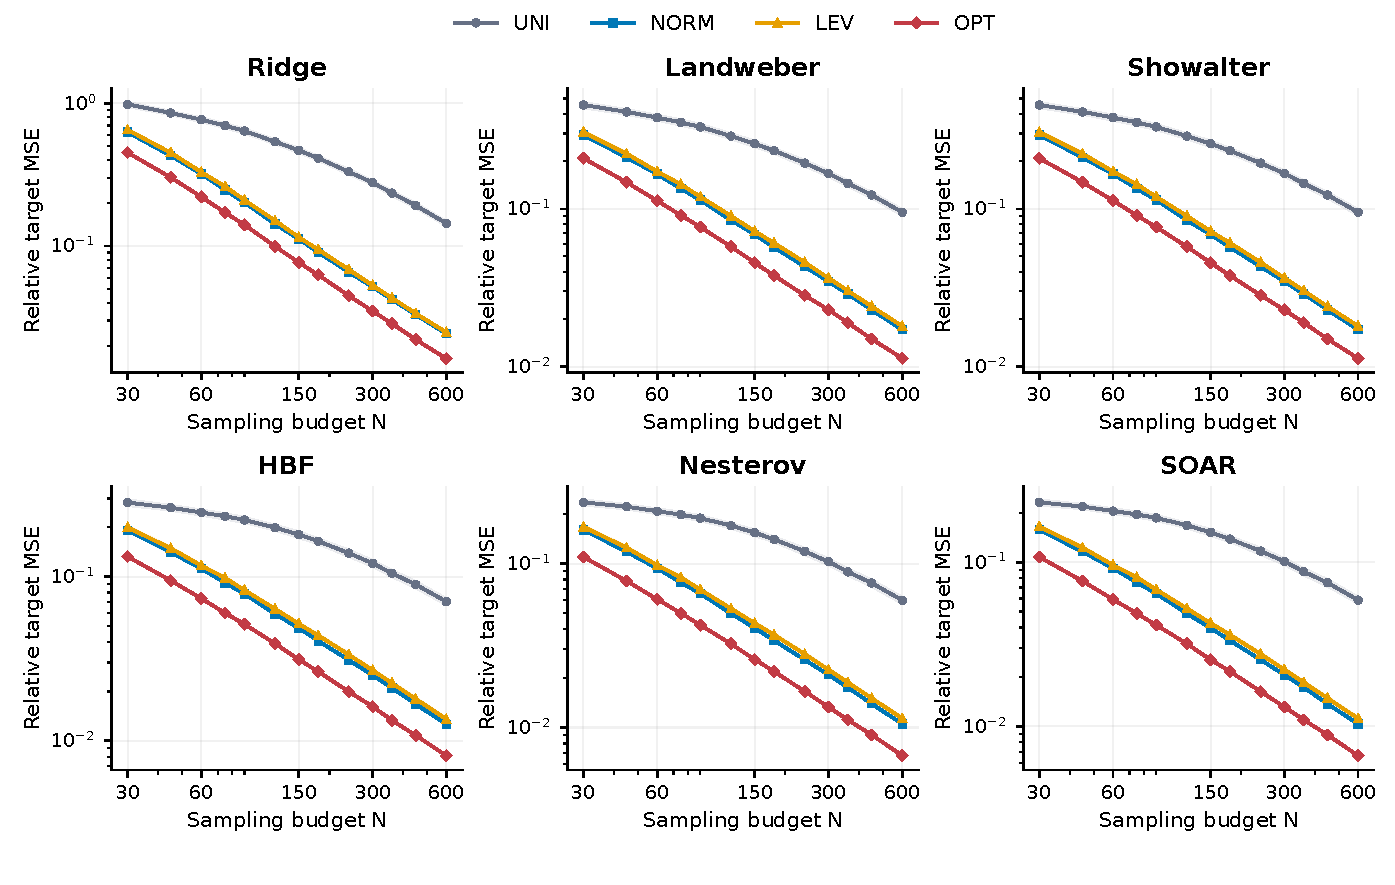
\includegraphics[width=.98\textwidth,trim=0 22bp 0 3bp,clip]{figures/01_target_approximation.pdf}
\caption{Native column probability comparisons: 40 independent data sets,
13 budgets, and 40 paired sketches per configuration. Each panel uses its own
fixed full-data numerical target. Lines are means and shading gives pointwise
95\% intervals across data-set means. Both axes are logarithmic.}
\label{fig:v7_probability_column}
\par\smallskip
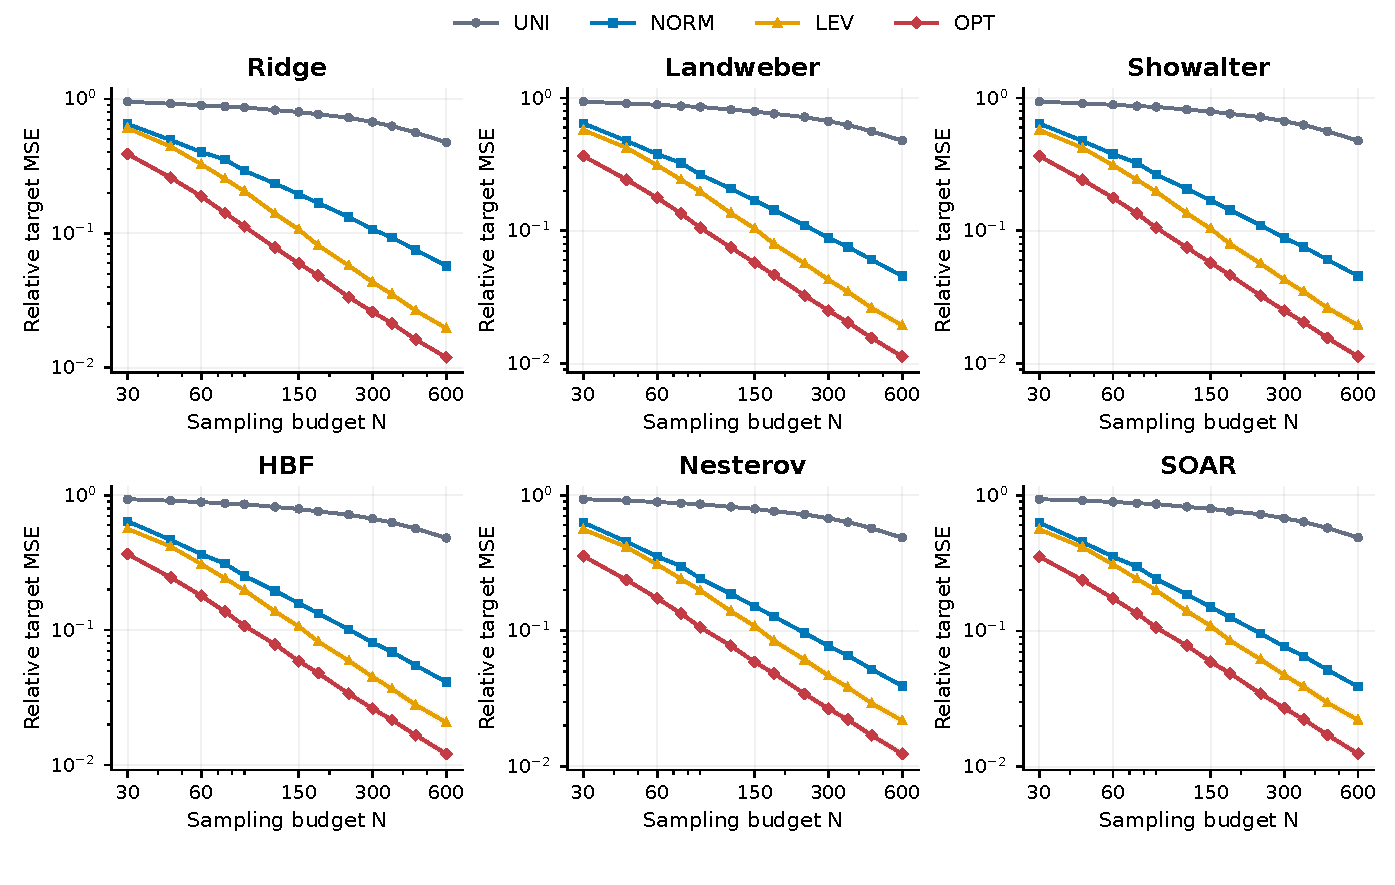
\includegraphics[width=.98\textwidth,trim=0 22bp 0 3bp,clip]{figures/r2_01_target_approximation.pdf}
\caption{Native row probability comparisons: 40 new independent spiked-row data sets,
13 budgets, and 40 paired sketches per configuration. Both Gram and response
cross-products are sampled. Targets and generator parameters are method-specific
and frozen. Shading gives pointwise 95\% intervals across data-set means;
both axes are logarithmic.}
\label{fig:v7_probability_row}
\end{figure*}

\begin{figure*}[!tp]\centering
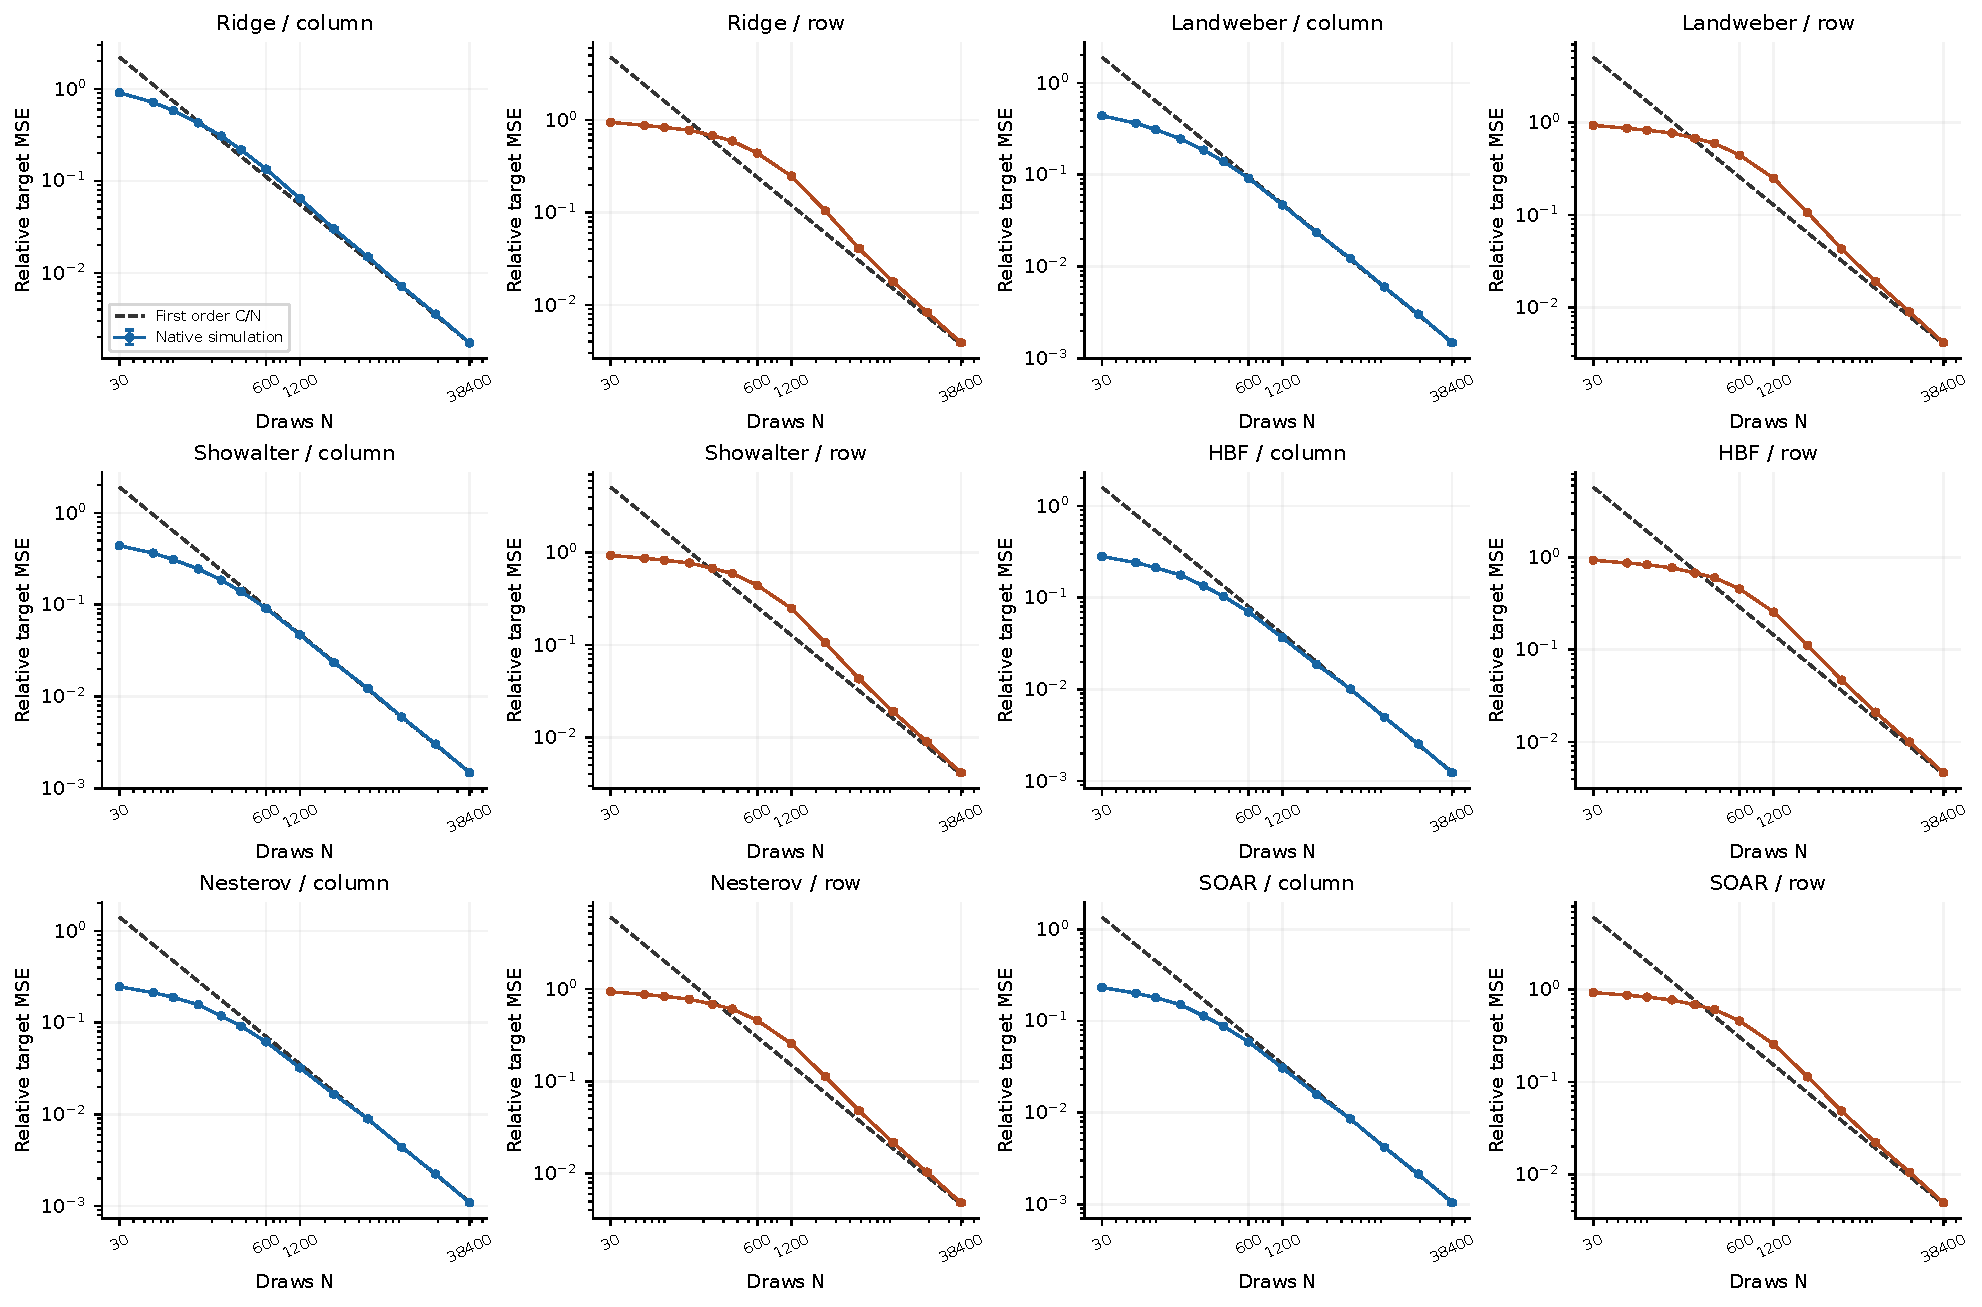
\includegraphics[width=.98\textwidth]{figures/r3_01_mse_absolute_compact.pdf}
\caption{Native Experiment III: empirical relative target MSE and the
first-order prediction $C_g/N$. Adjacent panels show column and row sampling
for each method. All 500 sketches contribute at each budget on the first
predesignated data set. Error bars are pointwise 95\% Monte Carlo intervals;
both axes are logarithmic.}
\label{fig:v7_absolute_mse}
\end{figure*}

\begin{figure*}[!tp]\centering
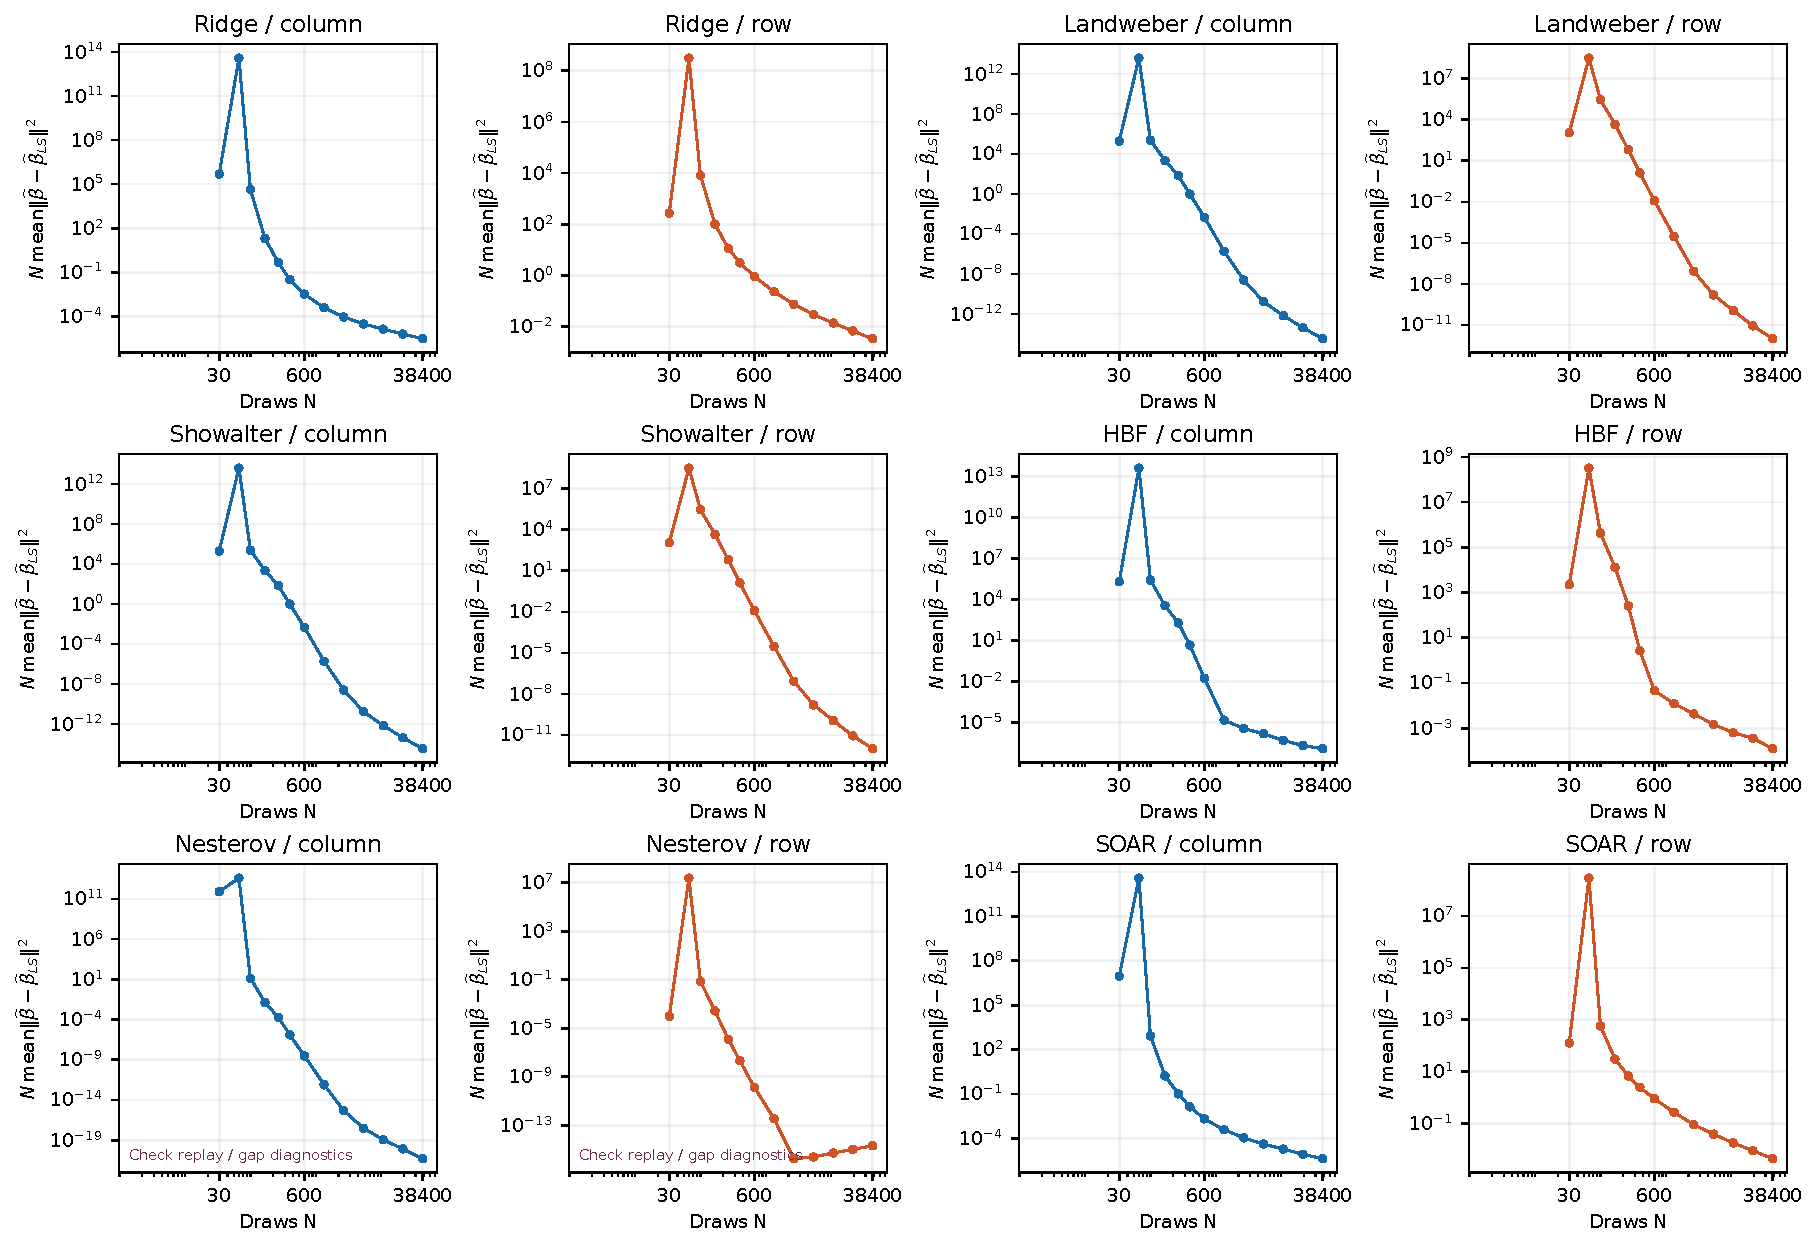
\includegraphics[width=.98\textwidth]{figures/r4_01_scaled_gap.pdf}
\caption{Actual native scaled squared gaps to same-draw QR LS, conditional on the first new data set in each direction. Each mean includes all 100 sketches. Vertical bars show pointwise 95\% Monte Carlo intervals where the lower endpoint is positive; full intervals are archived. High-budget Nesterov gaps are resolution-limited (Supplementary Table~\ref{supp-tab:exp4_replay}).}
\label{fig:v7_ls_gap}
\end{figure*}

\begin{figure*}[!tp]\centering
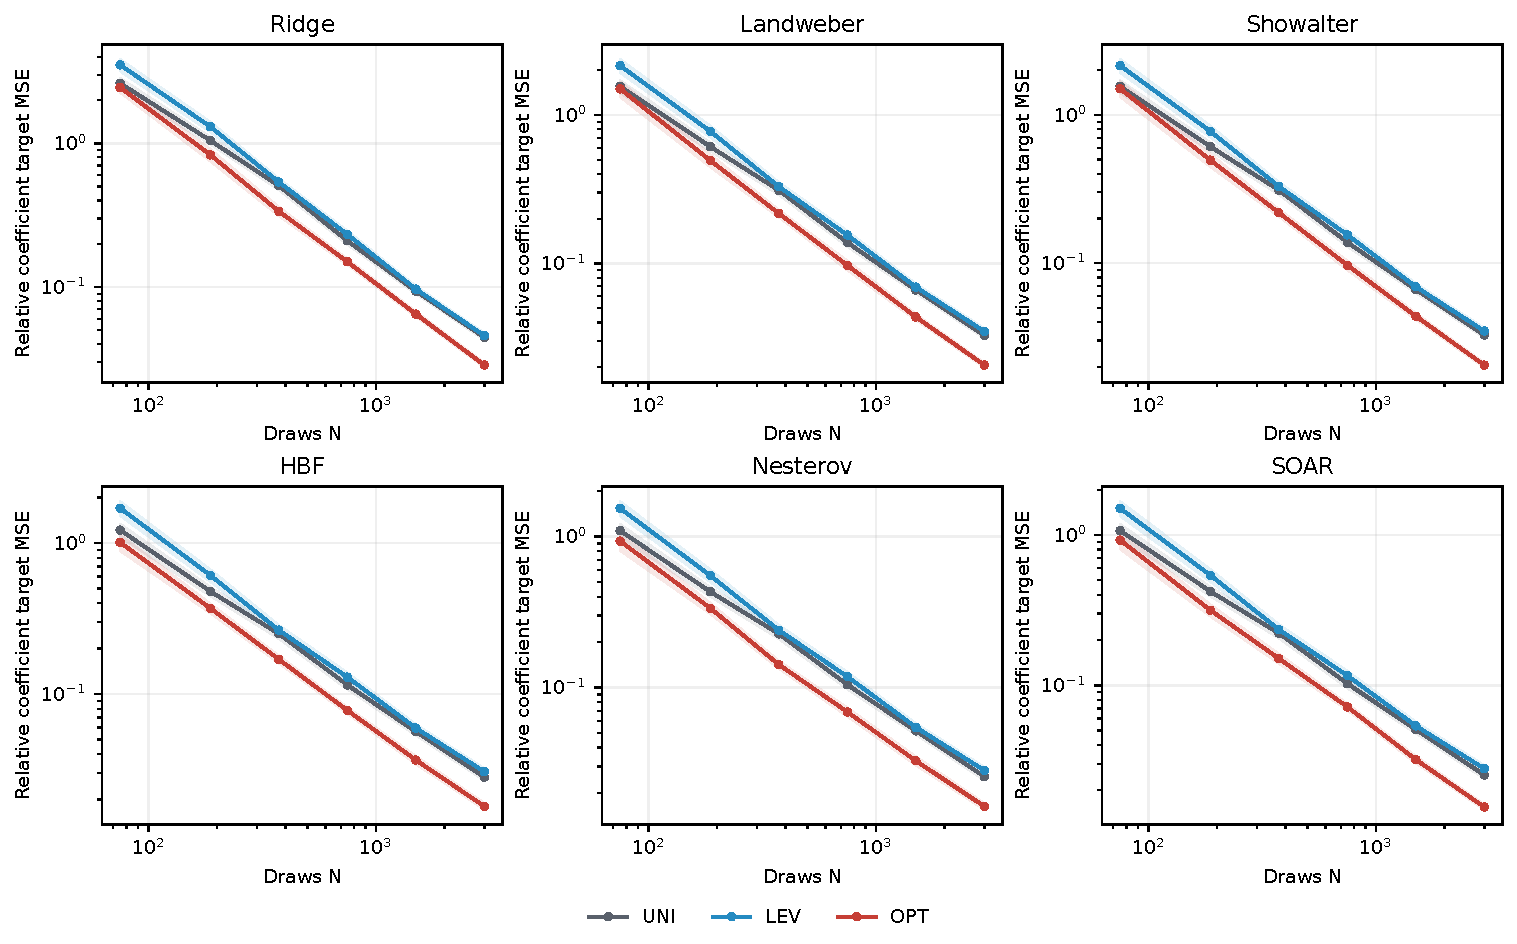
\includegraphics[width=.9\textwidth,height=.4\textheight,keepaspectratio]{figures/r5_01_gdsc_target.pdf}
\caption{Native GDSC full-coefficient target approximation, 30 paired draws per budget. All parameters, targets and probabilities are frozen before sampling. Shading gives conditional pointwise 95\% Monte Carlo intervals. NORM equals UNI.}
\label{fig:real_column_fixed}
\end{figure*}

\begin{figure*}[!tp]\centering
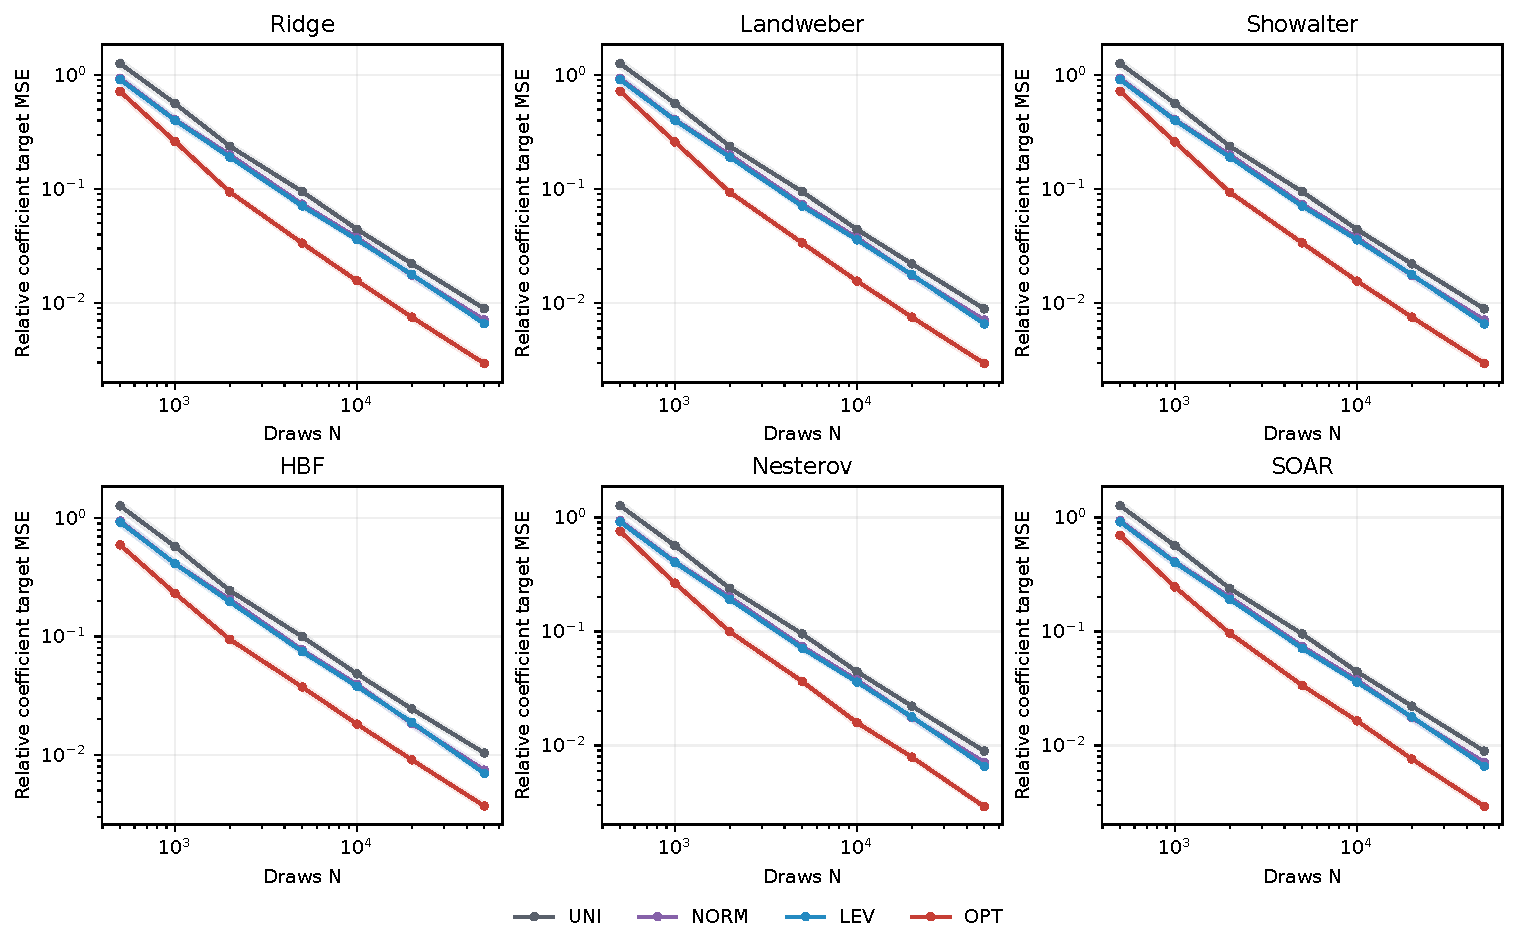
\includegraphics[width=.9\textwidth,height=.4\textheight,keepaspectratio]{figures/r5_02_year_target.pdf}
\caption{Native YearPredictionMSD row sampling, 50 paired draws per budget. Gram and response are jointly reweighted. Shading gives conditional pointwise 95\% Monte Carlo intervals; different methods retain their historical full-model parameter choices.}
\label{fig:real_row_fixed}
\end{figure*}

\subsection{Common Experimental Setup}
\label{subsec:v7_setup}
All six methods---Ridge, Landweber, Showalter, HBF, Nesterov, and SOAR---use
their actual computational outputs. Ridge is a direct-solve benchmark;
the other targets, estimates, and sensitivities use recurrences or fixed-grid
RK4 integration. Numerical flows and their derivatives use the same grid.
Column sampling retains full $X^\top u$ recovery, whereas row sampling
jointly reweights the Gram matrix and response cross-product.

The budget $N$ counts draws with replacement; the atom population has size
$N_0=p$ for columns and $N_0=n$ for rows. Each protocol fixes parameters,
iteration counts, and grids before sampling. These remain fixed across
rules and budgets in I--III and V; IV uses a prescribed budget-indexed path.
The common experimental calibration scale $\alpha_{\mathrm{exp}}$ is distinct
from a method's theoretical regularization parameter; full protocols write
this scale as $\alpha$.
UNI uses uniform probabilities, NORM uses squared norms, and LEV uses
leverage scores. OPT uses complete, response-dependent coefficient influences
with positive probability floors and is an oracle for the first-order
coefficient criterion.

We estimate the relative target MSE
\[
 \operatorname{RelMSE}_g(N)=
 \frac{\mathbb E_{\rm sub}\|\widehat\beta_{g,N}-\beta_g\|^2}{\|\beta_g\|^2},
\]
where $\beta_g$ is the method's full-data numerical output at the same
parameters as its sampled estimates. True-coefficient and prediction risks
are evaluated separately. The full protocols, auxiliary risks, sensitivity
analyses, and numerical checks are given in Supplementary
Sections~\ref{supp-supp:sec:native_common}--\ref{supp-supp:sec:native_exp5}.

\subsection{Experiment I: Native Column Subsampling Probabilities}
\label{subsec:exp_column_probabilities}
We generate 40 independent data sets with $n=60$, $p=1200$, heterogeneous
Gaussian columns, unit-norm Gaussian coefficients, and noise standard
deviation $0.5$. For each of 13 budgets from 30 to 600, we use 40 paired
sketches per rule. Parameters and probabilities are calibrated from the
complete data before sampling; Supplementary
Section~\ref{supp-supp:sec:native_exp1} specifies the design and calibration.

Errors are averaged over sketches within each data set and then across the
40 data sets. Figure~\ref{fig:v7_probability_column} shows pointwise 95\%
Student-$t_{39}$ intervals based on these independent data-set means.
OPT has the smallest mean in all 78 method--budget cells. At the prespecified
budget $N=150$, all 18 paired OPT-minus-baseline comparisons support lower
OPT error after Holm adjustment; OPT/NORM mean MSE ratios range from
0.640 to 0.684 (Supplementary Table~\ref{supp-tab:native_primary}).
Comparisons at other budgets are descriptive.


Average true risks exceed the zero-predictor reference in this noise
setting; the full-data targets have comparable risks.
Supplementary Section~\ref{supp-supp:sec:native_exp1} separates these risks
from target approximation and reports the tail and sensitivity analyses.

\subsection{Experiment II: Native Row Subsampling Probabilities}
\label{subsec:exp_row_probabilities}
We independently generate 40 spiked-row data sets with $n=1200$ and $p=60$.
The budget grid and 40 paired sketches per rule match Experiment I.
The same six methods use complete-data calibration and positive probability
floors, with both the Gram matrix and response cross-product jointly
reweighted. The data construction and coupled numerical influences are
specified in Supplementary Section~\ref{supp-supp:sec:native_exp2}.

Figure~\ref{fig:v7_probability_row} reports means and pointwise
Student-$t_{39}$ intervals across independent data-set means.
OPT has the smallest mean in all 78 method--budget cells.
At the prespecified budget $N=150$, all 18 paired comparisons support lower
OPT error after their own Holm correction; OPT/NORM mean target-MSE ratios
range from 0.305 to 0.394
(Supplementary Table~\ref{supp-tab:row_native_primary}).
Other budgets are descriptive. Separate true risks, sampled-row coverage,
tails, and robustness arms are reported in Supplementary
Section~\ref{supp-supp:sec:native_exp2}.


\subsection{Experiment III: Native First-Order MSE Calibration}
\label{subsec:v7_mse}
We independently generate 20 data sets in each sampling direction from the
models in Experiments I--II. Uniform sampling is used throughout, with the
same draws shared by all six methods. The predesignated first data set in
each direction uses 13 budgets from 30 to 38400 and 500 sketches per budget;
all 20 data sets are evaluated at $N=1200$ and $19200$.
The uniform-sampling calibration is fixed before any sketches, and full-data
targets and influences are recomputed at those parameters.

Let $J_i$ denote the complete coefficient influence of the actual numerical
map and $\bar J=N_0^{-1}\sum_iJ_i$, with $N_0=1200$.
The first-order relative MSE is $C_g/N$, where
\[
 C_g=\frac{N_0\sum_i\|J_i-\bar J\|^2}{\|\beta_g\|^2}.
\]
The constant is computed from the full-data algorithmic derivatives before
sampling, rather than fitted to the observed errors.

Figure~\ref{fig:v7_absolute_mse} compares the empirical MSE with $C_g/N$.
At $N=38400$, empirical-to-theoretical ratios range from 0.984 to 1.002 for
columns and from 1.032 to 1.039 for rows across the six methods. The intervals are
pointwise conditional Student-$t_{499}$ Monte Carlo intervals.
Full ratio curves, between-data-set variation, and the decomposition $e=Z+R$
are given in Supplementary Section~\ref{supp-supp:sec:native_exp3}.
A total ratio near one can coexist with a nonzero squared remainder and
an offsetting cross term. Budgets above 1200 examine the fixed-data limit.


\subsection{Experiment IV: Native Approximation to Same-Draw Least Squares}
\label{subsec:v7_ls}
Five fresh data sets per direction follow the models of I--II, with uniform
sampling. The predesignated first data set uses 100 sketches at 13 budgets
from 30 to 38400; the other four use 30 at $N=1200,19200$.
All six methods share each draw and its QR-based LS reference.
Complete data determine the budget-indexed parameter paths before sampling.
The algorithms execute every recurrence or RK4 update, and rank-deficient
draws and full column recovery are retained.
Supplementary Proposition~\ref{supp-prop:iv_rk4_bridge} verifies the finite-grid
RK4 residual and tail conditions in exact arithmetic under explicit spectral
bounds; floating-point precision is assessed separately by replay and grid
refinement.

For the actual coefficient outputs we report
\[
 D_g(N)=\frac NB\sum_{b=1}^B
 \|\widehat\beta_{g_N}^{(b)}-\widehat\beta_{\mathrm{LS}}^{(b)}\|^2.
\]
Figure~\ref{fig:v7_ls_gap} includes all outputs. All 12 direction--method
endpoint means on the first data set decrease from $N=1200$ to $38400$.
The high-budget Nesterov gaps are at the numerical resolution limit
(Supplementary Table~\ref{supp-tab:exp4_replay}).
Supplementary Section~\ref{supp-supp:sec:native_exp4} gives the paths,
implementation checks, low-budget tails, and separate true risks.
Budgets above 1200 examine the fixed-data limit.


\subsection{Experiment V: Native Real-Data Comparisons}
\label{subsec:real_data}
GDSC MG-132~\citep{yang2013gdsc} uses 749 training and 188 test cells
with 17,737 genes (column sampling). YearPredictionMSD~\citep{bertin2011year}
uses its official 463,715/51,630 training/test split and 90 features
(row sampling). Training-only preprocessing, historical splits, and
full-model tuning choices are fixed. Prior test exploration makes these
results descriptive; Supplementary
Section~\ref{supp-supp:subsec:real_protocol} documents their provenance and
the numerical parameters.

Figures~\ref{fig:real_column_fixed}--\ref{fig:real_row_fixed} report the
relative target MSE of Section~\ref{subsec:v7_setup}, estimated from
30 paired draws per budget for GDSC and 50 for YearPredictionMSD.
Targets and algorithmic-derivative OPT probabilities are fixed before
sampling. GDSC NORM equals UNI after standardization.
OPT attains the lowest mean target error in all 78 method--budget cells.
A two-sided reanalysis of the 36 comparisons at the prespecified budgets
749 and 5000 supports lower OPT error after one joint Holm correction
(largest adjusted $p<3\times10^{-8}$), conditional on the data and parameters.
The choice of sidedness was made in this reanalysis; the original one-sided
analysis and the frozen protocol are documented in Supplementary
Section~\ref{supp-supp:subsec:real_inference_revision}.
Prediction outcomes, including higher test error despite lower target
error for low-budget GDSC Ridge, are reported in Supplementary
Section~\ref{supp-supp:subsec:real_prediction}.


\FloatBarrier
\section{Conclusion}
\label{sec:conclusion}
The generator representation admits a common analysis of row and column
importance sampling while retaining their different influence functions.
Effective-space differentiation accommodates rank deficiency, and explicit
tail control yields expansions of the conditional moments in addition to distributional limits.
Residual comparison with sampled least squares handles changing
regularization, whereas fixed-target retuning retains its additional
first-order term. The growing-column results concern fixed-dimensional
contrasts under sufficient spectral conditions. The method-specific results
cover the stated recurrences and exact flows.
The native experiments use the actual numerical maps and their matching derivatives, with each sampled estimate compared to its full-data target at the same parameters. Influence sampling reduces mean fixed-target approximation error in the studied row and column settings. The MSE comparisons quantify finite-budget agreement with the first-order expansion, and the same-draw LS study combines exact-arithmetic verification of its finite-grid RK4 maps with floating-point resolution diagnostics.

\backmatter

\bmhead{Supplementary information}
Online Resource 1: Auxiliary lemmas, additional proofs, verification of the
accelerated and inertial generators, and detailed numerical protocols and diagnostics.

\section*{Statements and Declarations}

\bmhead{Funding}
This work was supported by the Shenzhen Sci-Tech Fund (Grant No. RCJC20231211090030059), National Natural Science Foundation of China (Grant No. 12171036), National Key Research and Development Program of China (Grant No. 2022YFC3310300) and Beijing Natural Science Foundation (Grant No. Z210001).

\bmhead{Competing interests}
The authors declare no competing interests.

\bmhead{Data and code availability}
Simulation inputs and results for Experiments I--IV and code for Experiments
I--V are publicly available at \href{https://github.com/L1wuyang/Subsampling}{\nolinkurl{github.com/L1wuyang/Subsampling}}.
GDSC data are available from Sanger (releases
\href{https://ftp.sanger.ac.uk/pub/project/cancerrxgene/releases/release-6.0/}{6.0}
and \href{https://ftp.sanger.ac.uk/pub/project/cancerrxgene/releases/release-8.4/}{8.4}),
and YearPredictionMSD from the
\href{https://doi.org/10.24432/C50K61}{UCI Machine Learning Repository}~\citep{bertin2011year}.
Data files, the repository version, and reproduction instructions are
specified in Supplementary Section~\ref{supp-supp:subsec:data_code}.

\bmhead{Author contributions}
Junchen Li and Ying-Ao Wang established the theoretical results, with Junchen Li
leading the development of the proofs. Junchen Li conducted the numerical experiments
under Ying-Ao Wang's guidance. Ye Zhang provided overall supervision.

\appendix
\numberwithin{equation}{section}
\section{Proofs of the core results}
\label{app:core-proofs}

This appendix proves Theorems~\ref{thm:fixed_generator},
\ref{thm:ls_equivalence}, \ref{thm:row_expansion},
\ref{thm:array_ls_clt}, and~\ref{thm:array_generator_clt}, and
Proposition~\ref{prop:optimal_probabilities}.
Auxiliary lemmas and additional proofs are in the supplementary material.

\subsection{Fixed-data expansion and exact moments}
\label{app:proof-fixed-generator}

\begin{proof}[Proof of Theorem~{\upshape\ref{thm:fixed_generator}}]
Let $B_N=\widehat M-M$ and use Supplementary Lemmas~\ref{supp-lem:local_matrix}
and~\ref{supp-lem:finite_atoms}. For columns the remainder is
\[
 R_N=X^\top\{g(H+B_N)-g(H)-Dg_H[B_N]\}Y.
\]
For rows, with $d_N=\widehat c-c$, the exact remainder is
\[
 \begin{aligned}
 R_N&=\{g(A+B_N)-g(A)-Dg_A[B_N]\}c\\
    &\quad +\{g(A+B_N)-g(A)\}d_N.
 \end{aligned}
\]
These identities also define $R_N$ outside $G_N$ by subtracting $Z_N$
from the actual error. On $G_N$, (A1) bounds the first matrix remainder
by $\epsilon(\|B_N\|_2)\|B_N\|_2$, where $\epsilon(t)\to0$ and is bounded
for $0\le t\le\delta$. Local differentiability bounds the second row term
by $C\|B_N\|_2\|d_N\|_2$.
The moment rates and $\Prob(G_N^c)\to0$ give $R_N=o_p(N^{-1/2})$.
Under (A2), the same bounds give $R_N=O_p(N^{-1})$.
The ordinary multivariate i.i.d.\ central limit theorem for the finite
influence distribution and Slutsky's theorem prove the stated, possibly
degenerate, Gaussian limit.

For the moment conclusions, the fourth-moment bound implies uniform
integrability of $N\|B_N\|_2^2$. Since $B_N\to_p0$,
\[
 N\,\E[\epsilon(\|B_N\|_2)^2\|B_N\|_2^2 \mathbf{1}_{G_N}]\longrightarrow0.
\]
Also, by Cauchy--Schwarz,
$\E(\|B_N\|_2^2\|d_N\|_2^2)=O(N^{-2})$.
Thus $N\,\E(\|R_N\|_2^2 \mathbf{1}_{G_N})\to0$.
The vector $Z_N$ is uniformly bounded over all samples because its
one-draw support is finite. Consequently, (A3) and the exponential
probability bound imply
\[
 \begin{aligned}
 N\,\E(\|R_N\|_2^2 \mathbf{1}_{G_N^c})
 &\le 2N\,\E(\|\widetilde\beta-\beta_g\|_2^2 \mathbf{1}_{G_N^c})\\
 &\quad +2N\,\E(\|Z_N\|_2^2 \mathbf{1}_{G_N^c})\longrightarrow0.
 \end{aligned}
\]
This proves the global $L^2$ remainder assertion.
Taking expectations and using Cauchy--Schwarz on the cross moments of
$Z_N$ and $R_N$ now proves the exact mean, covariance, and MSE expansions.

Under (A2), the good-event bound
$\|R_N\|_2\le C(\|B_N\|_2^2+\|B_N\|_2\|d_N\|_2)$
gives $\E(\|R_N\|_2 \mathbf{1}_{G_N})=O(N^{-1})$; omit $d_N$ for columns.
On the complement, (A3) and the exponential probability bound give
\[
 \begin{aligned}
 \E(\|R_N\|_2 \mathbf{1}_{G_N^c})
 &\le \{\E(\|\widetilde\beta-\beta_g\|_2^2 \mathbf{1}_{G_N^c})
                \Prob(G_N^c)\}^{1/2}\\
 &\quad +\E(\|Z_N\|_2 \mathbf{1}_{G_N^c})=o(N^{-1}).
 \end{aligned}
\]
Since $\E Z_N=0$, the asserted $O(N^{-1})$ bias follows.
\end{proof}

\subsection{Optimal sampling probabilities}
\label{app:proof-optimal-probabilities}

\begin{proof}[Proof of Proposition~{\upshape\ref{prop:optimal_probabilities}}]
Cauchy--Schwarz gives
$\sum_i w_i^2/\varpi_i\ge(\sum_iw_i)^2$. When at least one score is
positive, equality requires
$\varpi_i$ proportional to $w_i$ on the positive scores and no mass
elsewhere. This proves the unconstrained assertions, including the
nonattainment when zero and positive scores coexist.
For the lower-bound problem, the objective is convex. With a nonzero
score, its multiplier for the sum constraint is positive, and the
Karush--Kuhn--Tucker equations give $\varpi_i=\max\{\ell_i,\tau w_i\}$.
The normalization function is continuous, starts at $\sum_i\ell_i<1$,
and is strictly increasing after leaving that initial flat portion;
it therefore reaches $1$ at a unique $\tau$. Zero-score coordinates
are at their lower bounds, and strict convexity on positive-score
coordinates gives uniqueness. The all-zero and sole-feasible-vector
cases are immediate.
\end{proof}

\subsection{Equivalence to sampled least squares}
\label{app:proof-ls-equivalence}

\begin{proof}[Proof of Theorem~{\upshape\ref{thm:ls_equivalence}}]
All sample Gram ranges are contained in their respective full-data ranges.
On $G_{\mathsf{s},N}$ they coincide, and Weyl's inequality places the effective sample
spectrum in $I_\delta\subseteq I$, hence in the chosen window $\mathcal W$.
Consequently, on that event,
\[
 \begin{aligned}
 \norm{g_N(\widehat M_N)-\widehat M_N^\dagger}_{\rm eff}
       &\le 2\rho_N/m,\\
 \norm{\widehat\beta_{g_N,\mathsf{s}}-\widehat\beta_{{\rm LS},\mathsf{s}}}
       &\le C\rho_N.
 \end{aligned}
\]
The constant is independent of $g_N$: $X,Y$ are fixed, and
$\widehat c_N$ is uniformly bounded over all realizations.
Zero directions outside the full effective space vanish after back-projection,
or after multiplication by $\widehat c_N$.

On $G_{\mathsf{s},N}$, the inverse identity on the effective space gives a quadratic
remainder. Supplementary Lemma~\ref{supp-lem:finite_atoms} gives fourth moments of order $N^{-2}$.
On the complement, the same lemma bounds the pseudoinverse by $CN$ and gives
an exponentially small probability. Thus sampled least squares admits
\[
 \begin{aligned}
 \widehat\beta_{{\rm LS},\mathsf{s}}-\beta_{\rm LS}
   &=L_{{\rm LS},N}+R_{{\rm LS},N},\\
 \E L_{{\rm LS},N}&=0,\\
 \operatorname{Cov}(L_{{\rm LS},N})&=\Omega_{{\rm LS},\mathsf{s}}/N,\\
 \E\norm{R_{{\rm LS},N}}^2&=O(N^{-2}).
 \end{aligned}
\]
Differentiating the inverse gives column scores
$-\beta_{{\rm LS},j}P_{\cdot j}$, whose sum is $-\beta_{\rm LS}$,
and row scores $A^\dagger x_i e_i$, whose sum is zero because $X^\top e=0$.
This proves the covariance formulas. The finite-support central limit theorem
and the good-event comparison prove consistency and \eqref{eq:ls_clt}.

If $\sqrt N\,\rho_N\to0$, the squared comparison error on $G_{\mathsf{s},N}$ is
$o(N^{-1})$. On its complement, use \eqref{eq:ls_tail} and the polynomial
bound for sampled least squares. The comparison error is therefore
$o(N^{-1})$ in squared mean, proving \eqref{eq:ls_exact_moments}.
For the $O(N^{-1})$ bias, the good-event comparison has mean $O(N^{-1})$.
The bad-event mean is bounded by
\[
 \begin{aligned}
 &\{\E[\norm{\widehat\beta_{g_N,\mathsf{s}}-\beta_{\rm LS}}^2
                  \mathbf{1}_{G_{\mathsf{s},N}^c}]\Prob(G_{\mathsf{s},N}^c)\}^{1/2}\\
 &\qquad=o(N^{-1/2}e^{-cN/2}),
 \end{aligned}
\]
and the sampled-LS bias is $O(N^{-1})$.
\end{proof}

\subsection{Expansion under fixed-target retuning}
\label{app:proof-row-expansion}

\begin{proof}[Proof of Theorem~{\upshape\ref{thm:row_expansion}}]
On the high-probability event specified in the theorem, the exact identity
$G\widehat G^{-1}=I_{\mathcal R}+\Delta_N$ gives
$\widehat G=(I_{\mathcal R}+\Delta_N)^{-1}G$.
The Neumann expansion and
$\widehat c_N-c=O_p(N^{-1/2})$ yield
\[
 \widehat G\widehat c_N
 =(I_{\mathcal R}-\Delta_N+O_p(N^{-1}))
       \{\beta_\alpha+G(\widehat c_N-c)\},
\]
which proves \eqref{eq:row_expansion_general}. No commutation of $G$ and
$\widehat G$ has been used. The complement has probability tending to zero.
\end{proof}

\subsection{Least-squares-centered array contrasts}
\label{app:proof-array-ls}

\begin{proof}[Proof of Theorem~{\upshape\ref{thm:array_ls_clt}}]
The summands in \(E_N\) are centered and independent, so
\begin{equation}
 \mathbb E\|E_N\|_F^2=\frac{v_N}{N}.
 \label{eq:array_gram_second_moment}
\end{equation}
Moreover, the definition of \(C_{0,N}\) and the norm bound for
\(B_N^\dagger\) imply
\[
 d=\sum_j\pi_{Nj}\|C_{0,N}^{-1/2}\psi_{Nj}\|^2
 \le \frac{\kappa_N^2v_N}{m_N^4}.
\]
Consequently,
\[
 \frac{v_N}{Nm_N^2}
 \le \frac1d\left(\frac{\kappa_Nv_N}{\sqrt N\,m_N^3}\right)^2
 \longrightarrow0.
\]
On \(\mathcal G_N=\{\|E_N\|_2\le m_N/2\}\), all matrices preserve
\(\mathcal H_N\), and \(\widehat B_N\) is positive definite on that space,
with smallest restricted eigenvalue at least \(m_N/2\).
In particular, its range equals \(\mathcal H_N\). By
\eqref{eq:array_gram_second_moment},
\(\mathbb P(\mathcal G_N^c)\le4v_N/(Nm_N^2)\to0\).

Restricting the inverse identity to \(\mathcal H_N\) gives
\[
 \|\widehat B_N^\dagger-B_N^\dagger
       +B_N^\dagger E_NB_N^\dagger\|_2
 \le \frac{2\|E_N\|_F^2}{m_N^3}.
\]
The positive spectrum of \(\widehat B_N\) lies in
\([m_N/2,M_N+m_N/2]\), and hence
\[
 \|\{f_N(\widehat B_N)-\widehat B_N^\dagger\}P_N\|_2
 \le \frac{2\rho_N}{m_N}.
\]
Since \(T_N=T_NP_N\), the standardized error in
\eqref{eq:array_ls_limit} equals
\[
 \frac1{\sqrt N}\sum_{t=1}^N C_{0,N}^{-1/2}\psi_{NJ_{Nt}}+R_N,
 \]
where the remainder satisfies
\[
 \|R_N\|\mathbf{1}_{\mathcal G_N}
 \le2\sqrt N\,\kappa_N
       \left(\frac{\|E_N\|_F^2}{m_N^3}+\frac{\rho_N}{m_N}\right).
\]
The first contribution to this bound has expectation at most
\(2\kappa_Nv_N/(\sqrt N\,m_N^3)\); the second tends to zero by
\eqref{eq:array_ls_rates}. Thus \(R_N=o_p(1)\), including the complement
of \(\mathcal G_N\). The standardized summands have mean zero and
covariance \(I_d\). Their Lindeberg condition gives the multivariate
central limit theorem~\citep[Proposition~2.27]{vandervaart1998asymptotic},
and Slutsky's theorem completes the proof.
\end{proof}

\subsection{Generator-centered array contrasts}
\label{app:proof-array-generator}

\begin{proof}[Proof of Theorem~{\upshape\ref{thm:array_generator_clt}}]
By \eqref{eq:array_gram_second_moment}, the complement of
\(\{\|E_N\|_2\le\delta_N\}\) has probability at most
\(v_N/(N\delta_N^2)\to0\). On \(\{\|E_N\|_2\le\delta_N\}\) the assumed Taylor bound applies,
and the standardized error is
\(N^{-1/2}\sum_{t=1}^N C_{f,N}^{-1/2}\phi_{NJ_{Nt}}\) plus a remainder
bounded by \(\sqrt N\,\kappa_{f,N}K_N\|E_N\|_F^2\).
The expectation of this bound is
\(\kappa_{f,N}K_Nv_N/\sqrt N\to0\).
Linearity of \(\mathcal D_N\) gives centered influences, whose standardized
covariance is \(I_d\). Lindeberg and Slutsky again give the conclusion.
\end{proof}

% Bibliography style is supplied by sn-jnl.
\setlength{\bibsep}{3pt plus1pt minus0.5pt}
\bibliography{references}

\end{document}

